% Options for packages loaded elsewhere
\PassOptionsToPackage{unicode}{hyperref}
\PassOptionsToPackage{hyphens}{url}
\PassOptionsToPackage{dvipsnames,svgnames,x11names}{xcolor}
%
\documentclass[
  ignorenonframetext,
  aspectratio=169]{beamer}
\usepackage{pgfpages}
\setbeamertemplate{caption}[numbered]
\setbeamertemplate{caption label separator}{: }
\setbeamercolor{caption name}{fg=normal text.fg}
\beamertemplatenavigationsymbolsempty
% Prevent slide breaks in the middle of a paragraph
\widowpenalties 1 10000
\raggedbottom
\setbeamertemplate{part page}{
  \centering
  \begin{beamercolorbox}[sep=16pt,center]{part title}
    \usebeamerfont{part title}\insertpart\par
  \end{beamercolorbox}
}
\setbeamertemplate{section page}{
  \centering
  \begin{beamercolorbox}[sep=12pt,center]{part title}
    \usebeamerfont{section title}\insertsection\par
  \end{beamercolorbox}
}
\setbeamertemplate{subsection page}{
  \centering
  \begin{beamercolorbox}[sep=8pt,center]{part title}
    \usebeamerfont{subsection title}\insertsubsection\par
  \end{beamercolorbox}
}
\AtBeginPart{
  \frame{\partpage}
}
\AtBeginSection{
  \ifbibliography
  \else
    \frame{\sectionpage}
  \fi
}
\AtBeginSubsection{
  \frame{\subsectionpage}
}
\usepackage{amsmath,amssymb}
\usepackage{lmodern}
\usepackage{iftex}
\ifPDFTeX
  \usepackage[T1]{fontenc}
  \usepackage[utf8]{inputenc}
  \usepackage{textcomp} % provide euro and other symbols
\else % if luatex or xetex
  \usepackage{unicode-math}
  \defaultfontfeatures{Scale=MatchLowercase}
  \defaultfontfeatures[\rmfamily]{Ligatures=TeX,Scale=1}
\fi
\usetheme[]{CambridgeUS}
% Use upquote if available, for straight quotes in verbatim environments
\IfFileExists{upquote.sty}{\usepackage{upquote}}{}
\IfFileExists{microtype.sty}{% use microtype if available
  \usepackage[]{microtype}
  \UseMicrotypeSet[protrusion]{basicmath} % disable protrusion for tt fonts
}{}
\makeatletter
\@ifundefined{KOMAClassName}{% if non-KOMA class
  \IfFileExists{parskip.sty}{%
    \usepackage{parskip}
  }{% else
    \setlength{\parindent}{0pt}
    \setlength{\parskip}{6pt plus 2pt minus 1pt}}
}{% if KOMA class
  \KOMAoptions{parskip=half}}
\makeatother
\usepackage{xcolor}
\newif\ifbibliography
\usepackage{color}
\usepackage{fancyvrb}
\newcommand{\VerbBar}{|}
\newcommand{\VERB}{\Verb[commandchars=\\\{\}]}
\DefineVerbatimEnvironment{Highlighting}{Verbatim}{commandchars=\\\{\}}
% Add ',fontsize=\small' for more characters per line
\usepackage{framed}
\definecolor{shadecolor}{RGB}{248,248,248}
\newenvironment{Shaded}{\begin{snugshade}}{\end{snugshade}}
\newcommand{\AlertTok}[1]{\textcolor[rgb]{0.94,0.16,0.16}{#1}}
\newcommand{\AnnotationTok}[1]{\textcolor[rgb]{0.56,0.35,0.01}{\textbf{\textit{#1}}}}
\newcommand{\AttributeTok}[1]{\textcolor[rgb]{0.77,0.63,0.00}{#1}}
\newcommand{\BaseNTok}[1]{\textcolor[rgb]{0.00,0.00,0.81}{#1}}
\newcommand{\BuiltInTok}[1]{#1}
\newcommand{\CharTok}[1]{\textcolor[rgb]{0.31,0.60,0.02}{#1}}
\newcommand{\CommentTok}[1]{\textcolor[rgb]{0.56,0.35,0.01}{\textit{#1}}}
\newcommand{\CommentVarTok}[1]{\textcolor[rgb]{0.56,0.35,0.01}{\textbf{\textit{#1}}}}
\newcommand{\ConstantTok}[1]{\textcolor[rgb]{0.00,0.00,0.00}{#1}}
\newcommand{\ControlFlowTok}[1]{\textcolor[rgb]{0.13,0.29,0.53}{\textbf{#1}}}
\newcommand{\DataTypeTok}[1]{\textcolor[rgb]{0.13,0.29,0.53}{#1}}
\newcommand{\DecValTok}[1]{\textcolor[rgb]{0.00,0.00,0.81}{#1}}
\newcommand{\DocumentationTok}[1]{\textcolor[rgb]{0.56,0.35,0.01}{\textbf{\textit{#1}}}}
\newcommand{\ErrorTok}[1]{\textcolor[rgb]{0.64,0.00,0.00}{\textbf{#1}}}
\newcommand{\ExtensionTok}[1]{#1}
\newcommand{\FloatTok}[1]{\textcolor[rgb]{0.00,0.00,0.81}{#1}}
\newcommand{\FunctionTok}[1]{\textcolor[rgb]{0.00,0.00,0.00}{#1}}
\newcommand{\ImportTok}[1]{#1}
\newcommand{\InformationTok}[1]{\textcolor[rgb]{0.56,0.35,0.01}{\textbf{\textit{#1}}}}
\newcommand{\KeywordTok}[1]{\textcolor[rgb]{0.13,0.29,0.53}{\textbf{#1}}}
\newcommand{\NormalTok}[1]{#1}
\newcommand{\OperatorTok}[1]{\textcolor[rgb]{0.81,0.36,0.00}{\textbf{#1}}}
\newcommand{\OtherTok}[1]{\textcolor[rgb]{0.56,0.35,0.01}{#1}}
\newcommand{\PreprocessorTok}[1]{\textcolor[rgb]{0.56,0.35,0.01}{\textit{#1}}}
\newcommand{\RegionMarkerTok}[1]{#1}
\newcommand{\SpecialCharTok}[1]{\textcolor[rgb]{0.00,0.00,0.00}{#1}}
\newcommand{\SpecialStringTok}[1]{\textcolor[rgb]{0.31,0.60,0.02}{#1}}
\newcommand{\StringTok}[1]{\textcolor[rgb]{0.31,0.60,0.02}{#1}}
\newcommand{\VariableTok}[1]{\textcolor[rgb]{0.00,0.00,0.00}{#1}}
\newcommand{\VerbatimStringTok}[1]{\textcolor[rgb]{0.31,0.60,0.02}{#1}}
\newcommand{\WarningTok}[1]{\textcolor[rgb]{0.56,0.35,0.01}{\textbf{\textit{#1}}}}
\setlength{\emergencystretch}{3em} % prevent overfull lines
\providecommand{\tightlist}{%
  \setlength{\itemsep}{0pt}\setlength{\parskip}{0pt}}
\setcounter{secnumdepth}{-\maxdimen} % remove section numbering
\ifLuaTeX
\usepackage[bidi=basic]{babel}
\else
\usepackage[bidi=default]{babel}
\fi
\babelprovide[main,import]{spanish}
% get rid of language-specific shorthands (see #6817):
\let\LanguageShortHands\languageshorthands
\def\languageshorthands#1{}

%\usepackage[spanish,es-nolists]{babel}
%%\usepackage[spanish]{babel}
%% change fontsize of R code
%%colorines
\usepackage{amsmath,color,array,booktabs,algorithm2e}
%\newcommand\blue[1]{\textcolor{blue}{#1}}
%\newcommand\red[1]{\textcolor{red}{#1}}

%% change fontsize of output
\let\oldverbatim\verbatim
\let\endoldverbatim\endverbatim
\renewenvironment{verbatim}{\tiny\oldverbatim}{\endoldverbatim}

%\usepackage[table,xcdraw]{xcolor}

\usepackage{makecell}
 \usepackage{booktabs}
 \usepackage{adjustbox}
 \usepackage{amsmath,color,array,booktabs,algorithm2e}
 \newcommand\blue[1]{\textcolor{blue}{#1}}
 \newcommand\red[1]{\textcolor{red}{#1}}
 \setbeamertemplate{navigation symbols}{}
 \setbeamertemplate{footline}[page number]
 \usepackage{mathdots}
\usepackage{yhmath}
\usepackage{mathdots}
\usepackage{MnSymbol}
\renewcommand{\contentsname}{Índice}
\renewcommand{\chaptername}{Parte}
\renewcommand{\sectionname}{Sección}
\ifLuaTeX
  \usepackage{selnolig}  % disable illegal ligatures
\fi
\IfFileExists{bookmark.sty}{\usepackage{bookmark}}{\usepackage{hyperref}}
\IfFileExists{xurl.sty}{\usepackage{xurl}}{} % add URL line breaks if available
\urlstyle{same} % disable monospaced font for URLs
\hypersetup{
  pdftitle={R básico},
  pdflang={es-ES},
  colorlinks=true,
  linkcolor={Maroon},
  filecolor={Maroon},
  citecolor={Blue},
  urlcolor={Blue},
  pdfcreator={LaTeX via pandoc}}

\title{R básico}
\author{}
\date{\vspace{-2.5em}10-2022}

\begin{document}
\frame{\titlepage}

\begin{frame}[allowframebreaks]
  \tableofcontents[hideallsubsections]
\end{frame}
\hypertarget{analisis-de-datos-ordinales}{%
\section{Analisis de datos
ordinales}\label{analisis-de-datos-ordinales}}

\begin{frame}{Descripción de datos ordinales}
\protect\hypertarget{descripciuxf3n-de-datos-ordinales}{}
Los \blue{datos ordinales} son parecidos a los cualitativos, en el
sentido de que son cualidades de los individuos u objetos.

La diferencia existente entre los datos cualitativos y los ordinales
reside en las características que expresan. En el caso de los ordinales,
éstas tienen un orden natural que permite ``acumular'' observaciones.
\end{frame}

\begin{frame}{Frecuencias para datos ordinales}
\protect\hypertarget{frecuencias-para-datos-ordinales}{}
Al trabajar con datos ordinales, el orden de los niveles de los datos
nos permite calcular no solo frecuencias absolutas y relativas, sino
también \blue{frecuencias acumuladas}.

Es decir, podemos contar cuantas veces hemos observado un dato menor o
igual a este.
\end{frame}

\begin{frame}[fragile]{Ejemplo 1}
\protect\hypertarget{ejemplo-1}{}
\textbf{Ejemplo 1}

Suponed que tenemos una muestra de 15 estudiantes de los cuales sabemos
su nota en el examen de Estadística. Clasificamos todos estos resultados
en Suspenso (\(S\)), Aprobado (\(A\)), Notable (\(N\)) y Excelente
(\(Ex\)) y consideramos su orden natural \(S<A<N<Ex\).

Las notas obtenidas han sido las siguientes
\[S,\ A,\ N,\ Ex,\ S,\ S,\ Ex,\ Ex,\ N,\ A,\ A,\ A,\ A,\ N,\ S\]

Como recordaréis, para saber cuantas hay de cada una (su frecuencia
absoluta), utilizamos la función \texttt{table()}
\end{frame}

\begin{frame}[fragile]{Ejemplo 1}
\protect\hypertarget{ejemplo-1-1}{}
\begin{Shaded}
\begin{Highlighting}[]
\NormalTok{notas }\OtherTok{=} \FunctionTok{ordered}\NormalTok{(}\FunctionTok{c}\NormalTok{(}\StringTok{"S"}\NormalTok{,}\StringTok{"A"}\NormalTok{, }\StringTok{"N"}\NormalTok{, }\StringTok{"Ex"}\NormalTok{, }\StringTok{"S"}\NormalTok{, }\StringTok{"S"}\NormalTok{,}
                  \StringTok{"Ex"}\NormalTok{,}\StringTok{"Ex"}\NormalTok{, }\StringTok{"N"}\NormalTok{, }\StringTok{"A"}\NormalTok{, }\StringTok{"A"}\NormalTok{, }\StringTok{"A"}\NormalTok{,}
                  \StringTok{"A"}\NormalTok{, }\StringTok{"N"}\NormalTok{, }\StringTok{"S"}\NormalTok{),}
                \AttributeTok{levels =} \FunctionTok{c}\NormalTok{(}\StringTok{"S"}\NormalTok{, }\StringTok{"A"}\NormalTok{, }\StringTok{"N"}\NormalTok{, }\StringTok{"Ex"}\NormalTok{))}
\FunctionTok{table}\NormalTok{(notas)}
\end{Highlighting}
\end{Shaded}

\begin{verbatim}
## notas
##  S  A  N Ex 
##  4  5  3  3
\end{verbatim}

Como podréis observar, hay 4 \(S\), 5 \(A\), 3 \(N\) y 3 \(Ex\).
\end{frame}

\begin{frame}{Ejemplo 1}
\protect\hypertarget{ejemplo-1-2}{}
En lo referente a \textbf{frecuencias absolutas acumuladas}, hay

\begin{itemize}
\tightlist
\item
  4 estudiantes con \(S\) o menos. Ello implica que la frecuencia
  acumulada de \(S\) es 4
\item
  9 estudiantes que han obtenido \(A\) o menos. Entonces, la frecuencia
  acumulada de \(A\) es 9
\item
  12 estudiantes los cuales han obtenido \(N\) o menos. Así, la
  frecuencia acumulada de \(N\) es 12
\item
  15 estudiantes (todos) que han obtenido \(Ex\) o menos. De este modo,
  la frecuencia acumulada de \(Ex\) es 15, o sea, el total.
\end{itemize}
\end{frame}

\begin{frame}{Ejemplo 1}
\protect\hypertarget{ejemplo-1-3}{}
\blue{
Frecuencia relativa acumulada.
} Es la fracción del total de las observaciones en tanto por 1 que
representa su frecuencia absoluta acumulada

Así, las frecuencias relativas acumuladas respectivas son

\begin{itemize}
\tightlist
\item
  \(S:\ \frac{4}{15} \approx\) 0.27
\item
  \(A:\ \frac{9}{15}\approx\) 0.6
\item
  \(N:\ \frac{12}{15}\approx\) 0.8
\item
  \(Ex:\ \frac{15}{15}=1\)
\end{itemize}
\end{frame}

\begin{frame}{Frecuencia relativa acumulada}
\protect\hypertarget{frecuencia-relativa-acumulada}{}
En general, supongamos que realizamos \(n\) observaciones

\[x_1,\dots,x_n\]

de un cierto tipo de datos ordinales, cuyos posibles niveles ordenados
son

\[l_1<l_2<\dots<l_k\]

Por tanto, cada una de las observaciones \(x_j\) es igual a algún
\(l_i\). Diremos que todas estas observaciones forman una
\blue{variable ordinal}. En nuestro ejemplo anterior, los 4 niveles eran
\[S<A<N<Ex\]
\end{frame}

\begin{frame}{Frecuencia relativa acumulada}
\protect\hypertarget{frecuencia-relativa-acumulada-1}{}
Además, nuestro \(n = 15\) y nuestros \(x_1,\dots,x_{15}\) son las
calificaciones obtenidas por los alumnos.

De este modo, con estas notaciones

\begin{itemize}
\tightlist
\item
  Las definiciones de frecuencias absolutas \(n_j\) y las relativas
  \(f_j\), para cada nivel \(l_j\) son las mismas que en una variable
  cualitativa.
\item
  Las frecuencia absoluta acumulada del nivel \(l_j\) en esta variable
  ordinal es el número \(N_j\) de observaciones \(x_i\) tales que
  \(x_i\le l_j\). Es decir, \[N_j=\sum_{i=1}^jn_i\]
\end{itemize}
\end{frame}

\begin{frame}{Frecuencia relativa acumulada}
\protect\hypertarget{frecuencia-relativa-acumulada-2}{}
\begin{itemize}
\tightlist
\item
  La frecuencia relativa acumulada del nivel \(l_j\) en esta variable
  ordinal es la fracción en tanto por 1 \(F_j\) de observaciones \(x_i\)
  tales que \(x_i\le l_j\). Es decir,
  \[F_j=\frac{N_j}{n}=\sum_{i=1}^jf_i\]
\end{itemize}
\end{frame}

\begin{frame}[fragile]{Ejemplo 2}
\protect\hypertarget{ejemplo-2}{}
\textbf{Ejemplo 2}

En un estudio, a un grupo de clientes de un restaurante se les hizo la
siguiente pregunta:

``¿Estás contento con el trato ofrecido por los trabajadores del
establecimiento?''

Las posibles respuestas forman una escala ordinal con \(1<2<3<4<5\).

Supongamos que se recogieron las siguientes respuestas de 50 técnicos:

\begin{Shaded}
\begin{Highlighting}[]
\FunctionTok{set.seed}\NormalTok{(}\DecValTok{2018}\NormalTok{)}
\NormalTok{clientes }\OtherTok{=} \FunctionTok{sample}\NormalTok{(}\DecValTok{1}\SpecialCharTok{:}\DecValTok{5}\NormalTok{, }\DecValTok{50}\NormalTok{, }\AttributeTok{replace =} \ConstantTok{TRUE}\NormalTok{)}
\NormalTok{clientes}
\end{Highlighting}
\end{Shaded}

\begin{verbatim}
##  [1] 3 4 5 2 5 1 3 4 2 4 3 3 1 1 5 3 1 3 3 5 1 4 2 5 3 4 5 1 2 2 1 5 5 2 1 2 5 5
## [39] 2 1 2 1 3 2 1 2 3 3 1 2
\end{verbatim}

\begin{Shaded}
\begin{Highlighting}[]
\FunctionTok{set.seed}\NormalTok{(}\ConstantTok{NULL}\NormalTok{)}
\end{Highlighting}
\end{Shaded}
\end{frame}

\begin{frame}[fragile]{Ejemplo 2}
\protect\hypertarget{ejemplo-2-1}{}
En este caso tenemos 5 niveles (\(k=5\)) y 50 observaciones (\(n=50\))
que forman una variable ordinal a la que hemos llamado
\texttt{clientes}.

Hemos calculado todas sus frecuencias (absoluta, relativa, acumulada y
relativa acumulada) y las hemos representado en la siguiente tabla.

\begin{verbatim}
##   Absoluta Relativa Acumulada Rel. Acumulada
## 1       12     0.24        12           0.24
## 2       12     0.24        24           0.48
## 3       11     0.22        35           0.70
## 4        5     0.10        40           0.80
## 5       10     0.20        50           1.00
\end{verbatim}

\textbf{Ejercicio.} Calculad todas las frecuencias y comprobad que son
exactamente estas.
\end{frame}

\begin{frame}{Frecuencia relativa acumulada}
\protect\hypertarget{frecuencia-relativa-acumulada-3}{}
Los gráficos para frecuencias absolutas y relativas absolutas de
variables ordinales son exactamente los mismos que para las variables
cualitativas.

También podemos utilizar diagramas de barras para describir frecuencias
acumuladas: en este caso, la altura de cada barra debe ser igual a la
frecuencia acumulada del nivel respectivo. Además, estos niveles deben
de aparecer ordenados de manera ascendente, de forma que las alturas de
las barras también tengan un orden ascendente.

No obstante, se recomienda no hacer uso de diagramas circulares a la
hora de representar frecuencias acumuladas, debido a que éstos no
representan la información sobre la acumulación de datos de forma fácil
de entender a simple vista.
\end{frame}

\hypertarget{descripciuxf3n-de-datos-ordinales-con-r}{%
\section{Descripción de datos ordinales con
R}\label{descripciuxf3n-de-datos-ordinales-con-r}}

\begin{frame}[fragile]{Función cumsum()}
\protect\hypertarget{funciuxf3n-cumsum}{}
¿Recordáis la función \texttt{cumsum()}? Pues esta puede ser utilizada a
la hora de calcular frecuencias acumuladas.

Retomemos el ejemplo anterior de las notas de los estudiantes y
calculemos y representemos en un diagrama de barras las frecuencias
acumuladas de la muestra de notas.

\begin{Shaded}
\begin{Highlighting}[]
\NormalTok{notas}
\end{Highlighting}
\end{Shaded}

\begin{verbatim}
##  [1] S  A  N  Ex S  S  Ex Ex N  A  A  A  A  N  S 
## Levels: S < A < N < Ex
\end{verbatim}

\begin{Shaded}
\begin{Highlighting}[]
\NormalTok{fAbs }\OtherTok{=} \FunctionTok{table}\NormalTok{(notas) }\CommentTok{\#Frec. abs.}
\FunctionTok{cumsum}\NormalTok{(fAbs) }\CommentTok{\#Frec. abs. acumuladas}
\end{Highlighting}
\end{Shaded}

\begin{verbatim}
##  S  A  N Ex 
##  4  9 12 15
\end{verbatim}
\end{frame}

\begin{frame}[fragile]{Función cumsum()}
\protect\hypertarget{funciuxf3n-cumsum-1}{}
\begin{Shaded}
\begin{Highlighting}[]
\FunctionTok{cumsum}\NormalTok{(}\FunctionTok{prop.table}\NormalTok{(fAbs)) }\CommentTok{\#Frec. relativas acumuladas}
\end{Highlighting}
\end{Shaded}

\begin{verbatim}
##         S         A         N        Ex 
## 0.2666667 0.6000000 0.8000000 1.0000000
\end{verbatim}

\begin{Shaded}
\begin{Highlighting}[]
\FunctionTok{barplot}\NormalTok{(fAbs, }\AttributeTok{main =} \StringTok{"Diagrama de barras de frecuencias absolutas"}\NormalTok{)}
\end{Highlighting}
\end{Shaded}

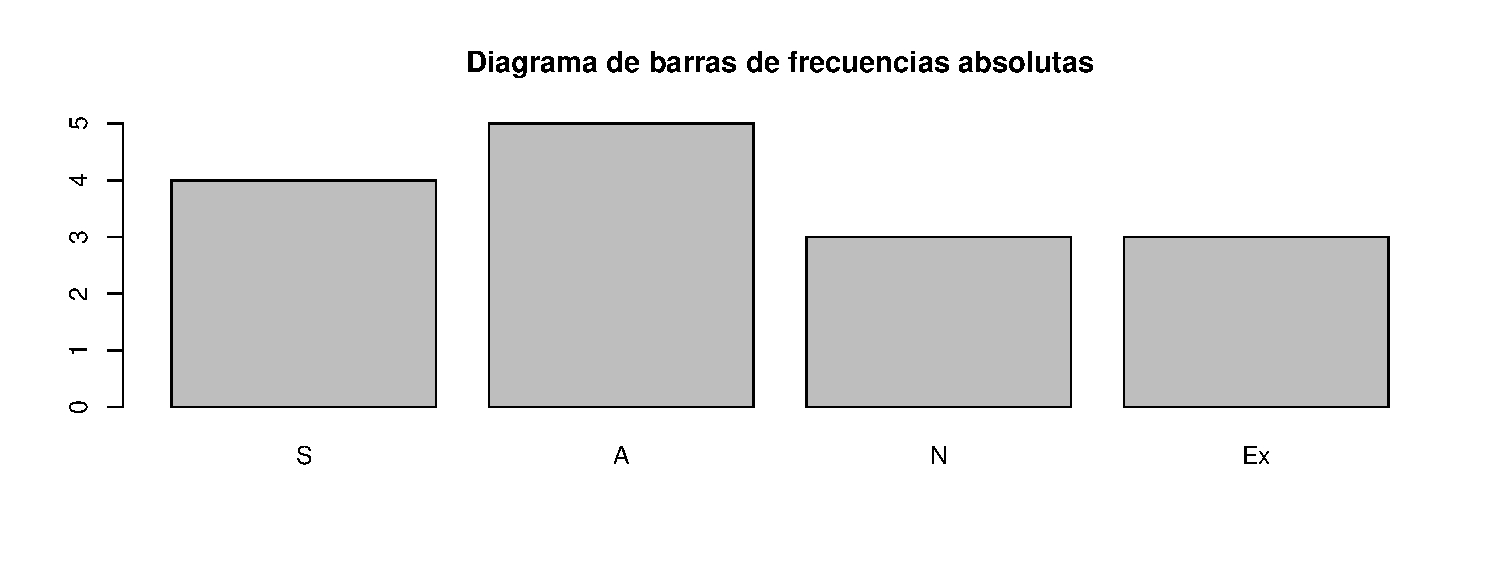
\includegraphics[width=0.8\linewidth]{Hora4_files/figure-beamer/unnamed-chunk-5-1}
\end{frame}

\begin{frame}[fragile]{Función cumsum()}
\protect\hypertarget{funciuxf3n-cumsum-2}{}
\begin{Shaded}
\begin{Highlighting}[]
\FunctionTok{barplot}\NormalTok{(}\FunctionTok{cumsum}\NormalTok{(fAbs), }\AttributeTok{main =} \StringTok{"Diagrama de barras de }
\StringTok{    frecuencias absolutas acumuladas"}\NormalTok{)}
\end{Highlighting}
\end{Shaded}

\begin{center}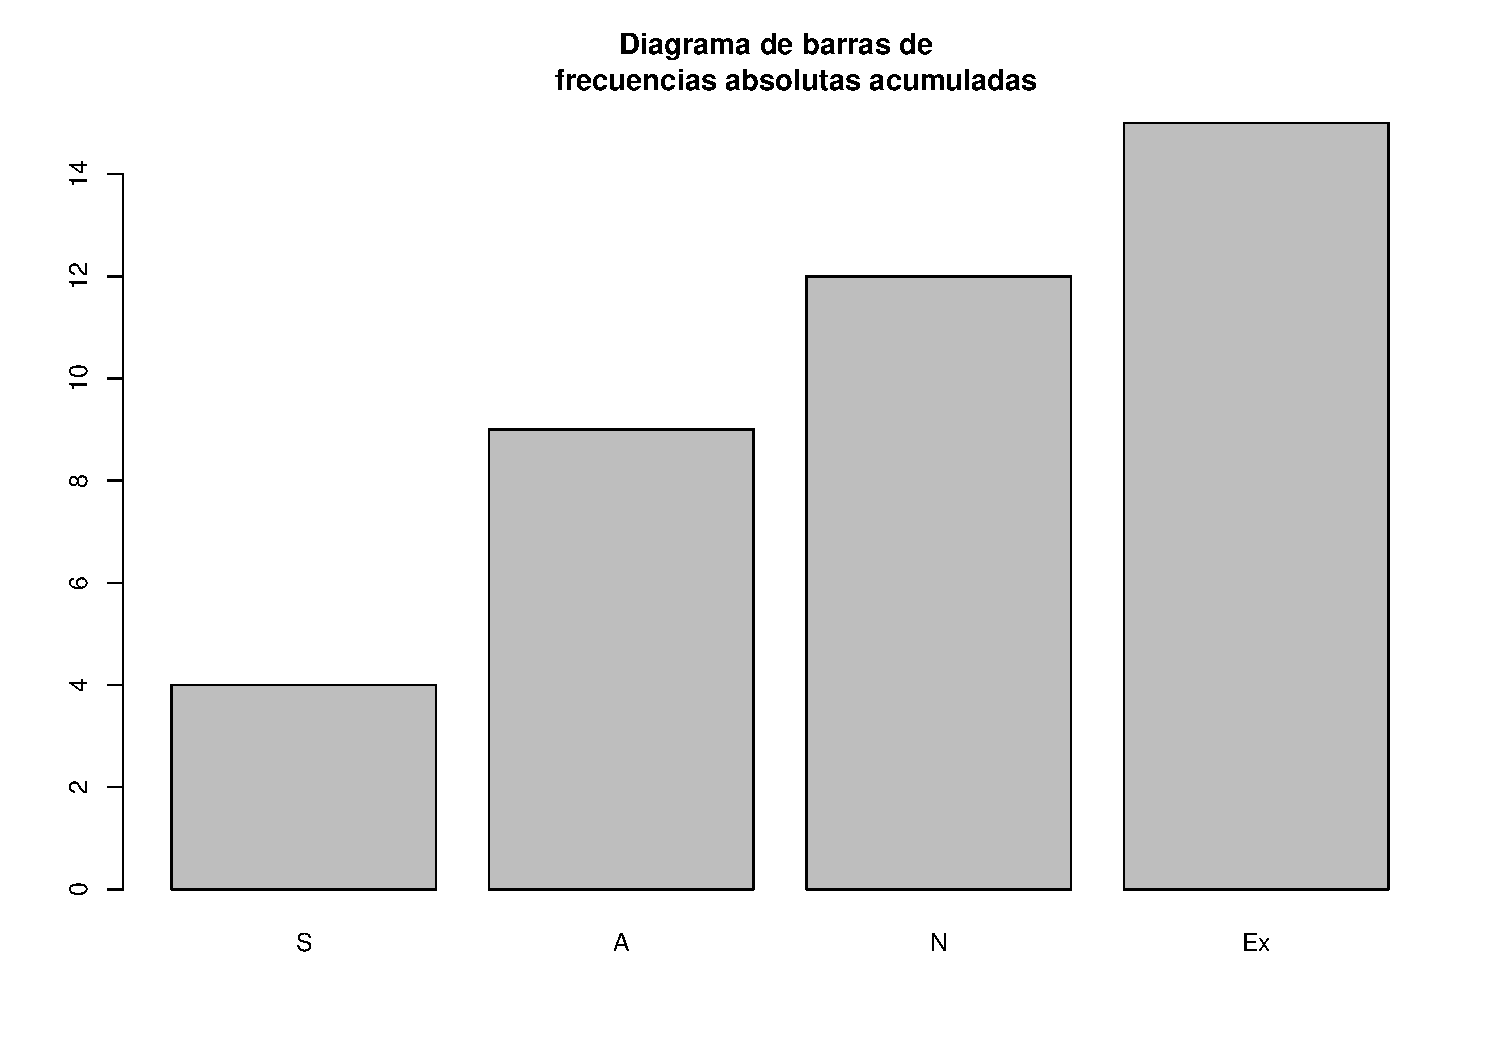
\includegraphics[width=250px]{Hora4_files/figure-beamer/unnamed-chunk-6-1} \end{center}
\end{frame}

\begin{frame}[fragile]{Función cumsum()}
\protect\hypertarget{funciuxf3n-cumsum-3}{}
Podríamos haber calculado las frecuencias relativas acumuladas de la
forma

\begin{Shaded}
\begin{Highlighting}[]
\FunctionTok{cumsum}\NormalTok{(}\FunctionTok{table}\NormalTok{(notas))}\SpecialCharTok{/}\FunctionTok{length}\NormalTok{(notas)}
\end{Highlighting}
\end{Shaded}

\begin{verbatim}
##         S         A         N        Ex 
## 0.2666667 0.6000000 0.8000000 1.0000000
\end{verbatim}

\begin{Shaded}
\begin{Highlighting}[]
\FunctionTok{cumsum}\NormalTok{(}\FunctionTok{table}\NormalTok{(notas)}\SpecialCharTok{/}\FunctionTok{length}\NormalTok{(notas))}
\end{Highlighting}
\end{Shaded}

\begin{verbatim}
##         S         A         N        Ex 
## 0.2666667 0.6000000 0.8000000 1.0000000
\end{verbatim}
\end{frame}

\begin{frame}[fragile]{Función cumsum()}
\protect\hypertarget{funciuxf3n-cumsum-4}{}
Pero no podemos hacer \texttt{prop.table(cumsum(table(notas)))}.

\textbf{Ejercicio.} Pensad qué ha entendido R que queríamos hacer con
esta última instrucción.
\end{frame}

\begin{frame}{Ejemplo 3}
\protect\hypertarget{ejemplo-3}{}
\textbf{Ejemplo 3}

Se ha evaluado el tamaño de los cuellos de 100 jirafas. Los niveles que
se han utilizado se los considera ordenados de la siguiente manera:

\[\text{Muy.corto}<\text{Corto}<\text{Normal}<\text{Largo}<\text{Muy.largo}\]

Los valores obtenidos en dicho estudio han sido los siguientes
\end{frame}

\begin{frame}[fragile]{Ejemplo 3}
\protect\hypertarget{ejemplo-3-1}{}
\begin{Shaded}
\begin{Highlighting}[]
\NormalTok{longitud}
\end{Highlighting}
\end{Shaded}

\begin{verbatim}
##   [1] Normal    Largo     Muy.largo Corto     Muy.largo Muy.corto Normal   
##   [8] Largo     Corto     Largo     Normal    Normal    Muy.corto Muy.corto
##  [15] Muy.largo Normal    Muy.corto Normal    Normal    Muy.largo Muy.corto
##  [22] Largo     Corto     Muy.largo Normal    Largo     Muy.largo Muy.corto
##  [29] Corto     Corto     Muy.corto Muy.largo Muy.largo Corto     Muy.corto
##  [36] Corto     Muy.largo Muy.largo Corto     Muy.corto Corto     Muy.corto
##  [43] Normal    Corto     Muy.corto Corto     Normal    Normal    Muy.corto
##  [50] Corto     Normal    Muy.corto Largo     Largo     Corto     Muy.corto
##  [57] Corto     Normal    Normal    Normal    Normal    Muy.corto Normal   
##  [64] Muy.corto Corto     Largo     Muy.corto Corto     Muy.corto Muy.largo
##  [71] Muy.corto Corto     Muy.largo Largo     Muy.largo Normal    Corto    
##  [78] Corto     Normal    Largo     Largo     Corto     Corto     Muy.largo
##  [85] Largo     Largo     Normal    Normal    Muy.corto Normal    Corto    
##  [92] Normal    Muy.corto Corto     Muy.corto Normal    Corto     Corto    
##  [99] Muy.corto Corto    
## Levels: Muy.corto < Corto < Normal < Largo < Muy.largo
\end{verbatim}
\end{frame}

\begin{frame}[fragile]{Ejemplo 3}
\protect\hypertarget{ejemplo-3-2}{}
Estudiemos sus frecuencias

\begin{Shaded}
\begin{Highlighting}[]
\NormalTok{Fr.Abs }\OtherTok{=} \FunctionTok{table}\NormalTok{(longitud)}
\NormalTok{Fr.Abs}
\end{Highlighting}
\end{Shaded}

\begin{verbatim}
## longitud
## Muy.corto     Corto    Normal     Largo Muy.largo 
##        23        26        24        13        14
\end{verbatim}

\begin{Shaded}
\begin{Highlighting}[]
\NormalTok{Fr.Rel }\OtherTok{=} \FunctionTok{prop.table}\NormalTok{(Fr.Abs)}
\NormalTok{Fr.Rel}
\end{Highlighting}
\end{Shaded}

\begin{verbatim}
## longitud
## Muy.corto     Corto    Normal     Largo Muy.largo 
##      0.23      0.26      0.24      0.13      0.14
\end{verbatim}
\end{frame}

\begin{frame}[fragile]{Ejemplo 3}
\protect\hypertarget{ejemplo-3-3}{}
\begin{Shaded}
\begin{Highlighting}[]
\NormalTok{Fr.Acum }\OtherTok{=} \FunctionTok{cumsum}\NormalTok{(Fr.Abs)}
\NormalTok{Fr.Acum}
\end{Highlighting}
\end{Shaded}

\begin{verbatim}
## Muy.corto     Corto    Normal     Largo Muy.largo 
##        23        49        73        86       100
\end{verbatim}

\begin{Shaded}
\begin{Highlighting}[]
\NormalTok{Fr.RAcum }\OtherTok{=} \FunctionTok{cumsum}\NormalTok{(Fr.Rel)}
\NormalTok{Fr.RAcum}
\end{Highlighting}
\end{Shaded}

\begin{verbatim}
## Muy.corto     Corto    Normal     Largo Muy.largo 
##      0.23      0.49      0.73      0.86      1.00
\end{verbatim}
\end{frame}

\begin{frame}[fragile]{Ejemplo 3}
\protect\hypertarget{ejemplo-3-4}{}
La instrucción \texttt{barplot} produce el siguiente diagrama de barras
de frecuencias relativas acumuladas

\begin{Shaded}
\begin{Highlighting}[]
\FunctionTok{barplot}\NormalTok{(Fr.RAcum, }\AttributeTok{main =} \StringTok{"Diagrama de frecuencias relativas acumuladas"}\NormalTok{)}
\end{Highlighting}
\end{Shaded}

\begin{center}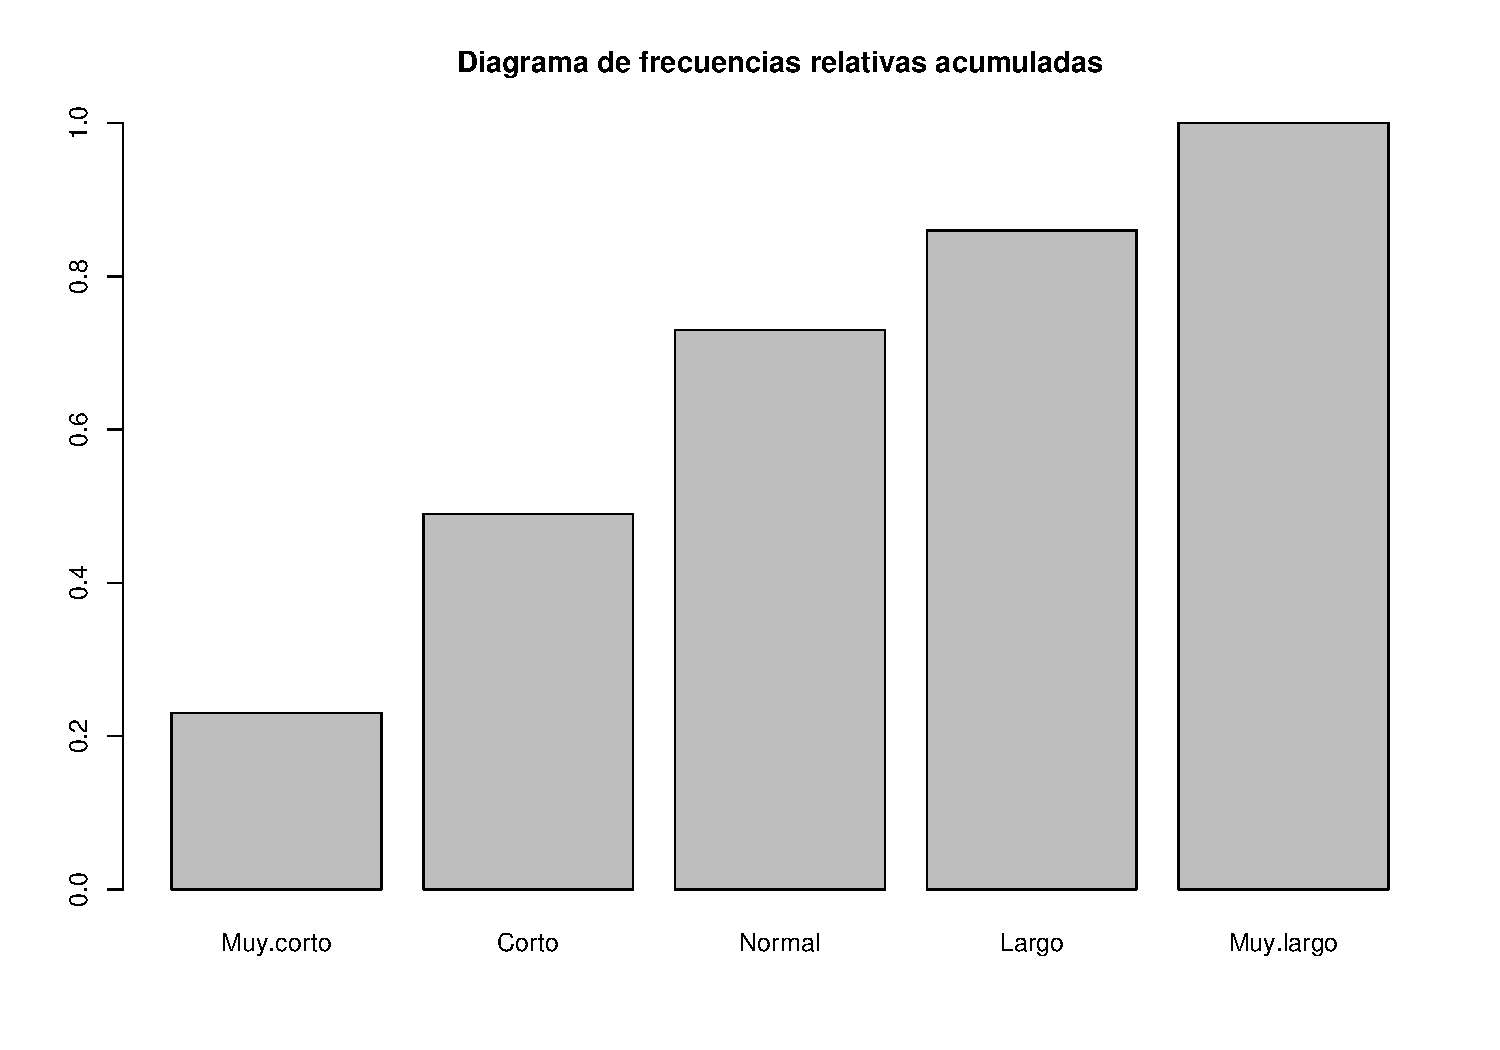
\includegraphics[width=225px]{Hora4_files/figure-beamer/unnamed-chunk-13-1} \end{center}
\end{frame}

\begin{frame}[fragile]{Función cumsum()}
\protect\hypertarget{funciuxf3n-cumsum-5}{}
Para calcular frecuencias acumuladas en una tabla multidimensional, hay
que aplicar a la tabla la función \texttt{cumsum} mediante la función
\texttt{apply} que ya explicábamos para matrices. En este caso en
concreto, la sintaxis de la instrucción sería

\texttt{apply(tabla,\ MARGIN=...,\ FUN=cumsum)}

donde el valor \texttt{MARGIN} ha de ser el de la dimensión en la que
queremos acumular las frecuencias: 1 si queremos hacerlo por filas, 2
para hacerlo por columnas, etc. Lo veremos todo más claro con un ejemplo
\end{frame}

\begin{frame}[fragile]{Ejemplo 4}
\protect\hypertarget{ejemplo-4}{}
\textbf{Ejemplo 4}

Supongamos que en el ejemplo anterior, el de las jirafas, estas
provienen de 4 zonas diferentes, A,B,C y D, de manera que las 30
primeras son de la zona A, las 25 siguientes de la B, las 35 siguientes
de la C y las 10 últimas de la D. Nos interesa estudiar la distribución
de las longitudes según la zona.

Vamos a organizar todos estos datos en un data frame llamado
\texttt{jirafas}. Para que nos sea más fácil visualizar la información,
es conveniente que las filas de las tablas de frecuencias correspondan a
las zonas. Por lo tanto, al definir el data frame, entraremos como
primera variable la de la muestra las zonas. Así, conseguiremos que
éstas aparezcan en las filas al aplicarle la función table.
\end{frame}

\begin{frame}[fragile]{Ejemplo 4}
\protect\hypertarget{ejemplo-4-1}{}
\begin{Shaded}
\begin{Highlighting}[]
\NormalTok{zonas }\OtherTok{=} \FunctionTok{rep}\NormalTok{(}\FunctionTok{c}\NormalTok{(}\StringTok{"A"}\NormalTok{,}\StringTok{"B"}\NormalTok{,}\StringTok{"C"}\NormalTok{,}\StringTok{"D"}\NormalTok{), }\FunctionTok{c}\NormalTok{(}\DecValTok{30}\NormalTok{,}\DecValTok{25}\NormalTok{,}\DecValTok{35}\NormalTok{,}\DecValTok{10}\NormalTok{))}
\NormalTok{jirafas }\OtherTok{=} \FunctionTok{data.frame}\NormalTok{(zonas,longitud)}
\FunctionTok{str}\NormalTok{(jirafas)}
\end{Highlighting}
\end{Shaded}

\begin{verbatim}
## 'data.frame':    100 obs. of  2 variables:
##  $ zonas   : chr  "A" "A" "A" "A" ...
##  $ longitud: Ord.factor w/ 5 levels "Muy.corto"<"Corto"<..: 3 4 5 2 5 1 3 4 2 4 ...
\end{verbatim}

\begin{Shaded}
\begin{Highlighting}[]
\FunctionTok{head}\NormalTok{(jirafas)}
\end{Highlighting}
\end{Shaded}

\begin{verbatim}
##   zonas  longitud
## 1     A    Normal
## 2     A     Largo
## 3     A Muy.largo
## 4     A     Corto
## 5     A Muy.largo
## 6     A Muy.corto
\end{verbatim}
\end{frame}

\begin{frame}[fragile]{Ejemplo 4}
\protect\hypertarget{ejemplo-4-2}{}
Para calcular la tabla de frecuencias absolutas acumuladas de las
longitudes por zonas y como las zonas definen las filas de la tabla
anterior, debemos utilizar la función \texttt{apply} con
\texttt{MARGIN\ =\ 1}.

\begin{Shaded}
\begin{Highlighting}[]
\FunctionTok{apply}\NormalTok{(}\FunctionTok{table}\NormalTok{(jirafas), }\AttributeTok{MARGIN =} \DecValTok{1}\NormalTok{, }\AttributeTok{FUN =}\NormalTok{ cumsum)}
\end{Highlighting}
\end{Shaded}

\begin{verbatim}
##            zonas
## longitud     A  B  C  D
##   Muy.corto  6  7  7  3
##   Corto     11 15 15  8
##   Normal    19 19 25 10
##   Largo     24 21 31 10
##   Muy.largo 30 25 35 10
\end{verbatim}
\end{frame}

\begin{frame}[fragile]{Ejemplo 4}
\protect\hypertarget{ejemplo-4-3}{}
Fijaos que la tabla se ha traspuesto. Resulta que cuando se aplica
\texttt{apply} a una \texttt{table} bidimensional, R intercambia, en
caso de ser necesario, filas por columnas en el resultado para que la
dimensión de la tabla resultante en la que se haya aplicado la función
sea la de las columnas.

Con lo cual, para volver a tener las zonas en las filas, hay que
trasponer el resultado de la función \texttt{apply}.

\begin{Shaded}
\begin{Highlighting}[]
\FunctionTok{t}\NormalTok{(}\FunctionTok{apply}\NormalTok{(}\FunctionTok{table}\NormalTok{(jirafas), }\AttributeTok{MARGIN =} \DecValTok{1}\NormalTok{, }\AttributeTok{FUN =}\NormalTok{ cumsum))}
\end{Highlighting}
\end{Shaded}

\begin{verbatim}
##      longitud
## zonas Muy.corto Corto Normal Largo Muy.largo
##     A         6    11     19    24        30
##     B         7    15     19    21        25
##     C         7    15     25    31        35
##     D         3     8     10    10        10
\end{verbatim}
\end{frame}

\begin{frame}[fragile]{Ejemplo 4}
\protect\hypertarget{ejemplo-4-4}{}
Vamos ahora a calcular la tabla de frecuencias relativas acumuladas de
las longitudes de cuello por zonas. Para conseguirlo, y en una única
instrucción, primero calculamos la tabla de frecuencias relativas por
filas, a continuación, con las funciones \texttt{apply} y
\texttt{cumsum} las acumulamos y, finalmente, trasponemos el resultado.

\begin{Shaded}
\begin{Highlighting}[]
\FunctionTok{t}\NormalTok{(}\FunctionTok{apply}\NormalTok{(}\FunctionTok{prop.table}\NormalTok{(}\FunctionTok{table}\NormalTok{(jirafas),}
                   \AttributeTok{margin =} \DecValTok{1}\NormalTok{), }
        \AttributeTok{MARGIN =} \DecValTok{1}\NormalTok{, }\AttributeTok{FUN =}\NormalTok{ cumsum))}
\end{Highlighting}
\end{Shaded}

\begin{verbatim}
##      longitud
## zonas Muy.corto     Corto    Normal     Largo Muy.largo
##     A      0.20 0.3666667 0.6333333 0.8000000         1
##     B      0.28 0.6000000 0.7600000 0.8400000         1
##     C      0.20 0.4285714 0.7142857 0.8857143         1
##     D      0.30 0.8000000 1.0000000 1.0000000         1
\end{verbatim}
\end{frame}

\begin{frame}[fragile]{Ejemplo 4}
\protect\hypertarget{ejemplo-4-5}{}
Vamos ahora a dibujar el diagrama de barras por bloques de esta tabla.
Nos interesa que las barras de este diagrama se agrupen por zonas.
Entonces, tendremos que aplicar \texttt{barplot} a la tabla sin
trasponer.

Además, vamos a colocar la leyenda en la esquina superior izquierda para
que no se superponga a ninguna barra. También reduciremos el tamaño del
texto de la leyenda para que quepa completamente.
\end{frame}

\begin{frame}[fragile]{Ejemplo 4}
\protect\hypertarget{ejemplo-4-6}{}
\begin{Shaded}
\begin{Highlighting}[]
\NormalTok{Diagrama }\OtherTok{=} \FunctionTok{apply}\NormalTok{(}\FunctionTok{prop.table}\NormalTok{(}\FunctionTok{table}\NormalTok{(jirafas), }\AttributeTok{margin =} \DecValTok{1}\NormalTok{),}
                 \AttributeTok{MARGIN =} \DecValTok{1}\NormalTok{, }\AttributeTok{FUN =}\NormalTok{ cumsum)}
\FunctionTok{barplot}\NormalTok{(Diagrama, }\AttributeTok{beside =} \ConstantTok{TRUE}\NormalTok{, }\AttributeTok{legend =} \ConstantTok{TRUE}\NormalTok{,}
\AttributeTok{main =} \StringTok{"Diagrama de barras de frecuencias relativas acumuladas }
\StringTok{        de longitudes por zonas"}\NormalTok{,}
\AttributeTok{args.legend=}\FunctionTok{list}\NormalTok{(}\AttributeTok{x=}\StringTok{"topleft"}\NormalTok{, }\AttributeTok{cex=}\FloatTok{0.55}\NormalTok{))}
\end{Highlighting}
\end{Shaded}
\end{frame}

\begin{frame}{Ejemplo 4}
\protect\hypertarget{ejemplo-4-7}{}
\begin{center}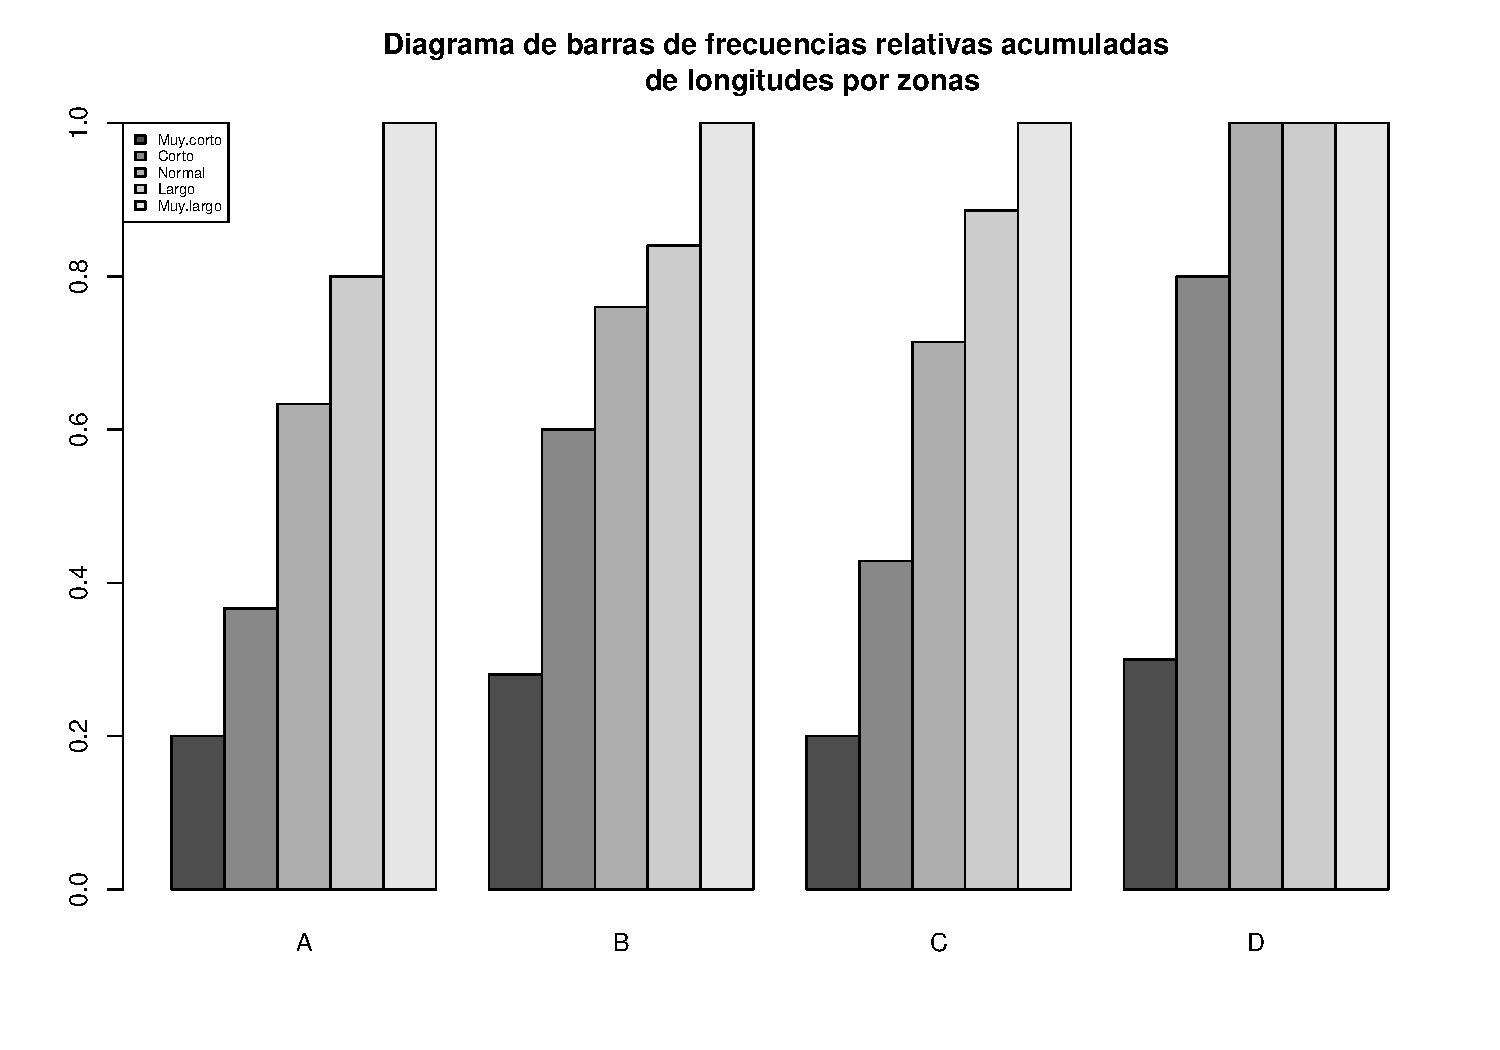
\includegraphics[width=300px]{Hora4_files/figure-beamer/unnamed-chunk-19-1} \end{center}
\end{frame}

\begin{frame}[fragile]{Ejemplo 5}
\protect\hypertarget{ejemplo-5}{}
\textbf{Ejemplo 5}

Consideremos el data frame \texttt{datacrab} y arreglemos los datos.

\begin{Shaded}
\begin{Highlighting}[]
\NormalTok{crabs }\OtherTok{=} \FunctionTok{read.table}\NormalTok{(}\StringTok{"../data/datacrab.txt"}\NormalTok{, }\AttributeTok{header =} \ConstantTok{TRUE}\NormalTok{)}
\NormalTok{crabs }\OtherTok{=}\NormalTok{ crabs[,}\SpecialCharTok{{-}}\DecValTok{1}\NormalTok{] }\CommentTok{\#Omitimos la primera columna}
\FunctionTok{str}\NormalTok{(crabs)}
\end{Highlighting}
\end{Shaded}

\begin{verbatim}
## 'data.frame':    173 obs. of  5 variables:
##  $ color : int  3 4 2 4 4 3 2 4 3 4 ...
##  $ spine : int  3 3 1 3 3 3 1 2 1 3 ...
##  $ width : num  28.3 22.5 26 24.8 26 23.8 26.5 24.7 23.7 25.6 ...
##  $ satell: int  8 0 9 0 4 0 0 0 0 0 ...
##  $ weight: int  3050 1550 2300 2100 2600 2100 2350 1900 1950 2150 ...
\end{verbatim}

La variable numérica \texttt{width} contiene la anchura de cada cangrejo
\end{frame}

\begin{frame}[fragile]{Ejemplo 5}
\protect\hypertarget{ejemplo-5-1}{}
\begin{Shaded}
\begin{Highlighting}[]
\FunctionTok{table}\NormalTok{(crabs}\SpecialCharTok{$}\NormalTok{width)}
\end{Highlighting}
\end{Shaded}

\begin{verbatim}
## 
##   21   22 22.5 22.9   23 23.1 23.2 23.4 23.5 23.7 23.8 23.9   24 24.1 24.2 24.3 
##    1    1    3    3    2    3    1    1    1    3    3    1    2    1    2    2 
## 24.5 24.7 24.8 24.9   25 25.1 25.2 25.3 25.4 25.5 25.6 25.7 25.8 25.9   26 26.1 
##    7    5    1    3    6    2    2    1    3    3    2    6    7    1    6    2 
## 26.2 26.3 26.5 26.7 26.8   27 27.1 27.2 27.3 27.4 27.5 27.6 27.7 27.8 27.9   28 
##    8    1    6    3    3    5    2    2    1    3    6    1    2    2    2    3 
## 28.2 28.3 28.4 28.5 28.7 28.9   29 29.3 29.5 29.7 29.8   30 30.2 30.3 30.5 31.7 
##    4    3    2    4    2    1    6    2    1    1    1    3    1    1    1    1 
## 31.9 33.5 
##    1    1
\end{verbatim}
\end{frame}

\begin{frame}[fragile]{Ejemplo 5}
\protect\hypertarget{ejemplo-5-2}{}
Vamos a convertir a la variable \texttt{width} en una variable ordinal
que agrupe las entradas de la variable original en niveles.

La manera más sencilla de llevarlo a cabo es utilizando la función
\texttt{cut}, que estudiaremos en detalle en lecciones posteriores. Por
ahora, basta con saber que la instrucción dividirá el vector numérico
\texttt{crabs\$width} en intervalos de extremos los puntos especificados
en el argumento \texttt{breaks}. El parámetro \texttt{right\ =\ FALSE}
sirve para indicar que los puntos de corte pertenecen la intervalo de su
derecha, e \texttt{Inf} indica \(\infty\).

Por lo tanto, nosotros llevaremos a cabo la siguiente instrucción

\begin{Shaded}
\begin{Highlighting}[]
\NormalTok{intervalos }\OtherTok{=} \FunctionTok{cut}\NormalTok{(crabs}\SpecialCharTok{$}\NormalTok{width, }\AttributeTok{breaks =} \FunctionTok{c}\NormalTok{(}\DecValTok{21}\NormalTok{,}\DecValTok{25}\NormalTok{,}\DecValTok{29}\NormalTok{,}\DecValTok{33}\NormalTok{,}\ConstantTok{Inf}\NormalTok{), }\AttributeTok{right =} \ConstantTok{FALSE}\NormalTok{, }
                 \AttributeTok{labels =} \FunctionTok{c}\NormalTok{(}\StringTok{"21{-}25"}\NormalTok{, }\StringTok{"25{-}29"}\NormalTok{, }\StringTok{"29{-}33"}\NormalTok{, }\StringTok{"33{-}..."}\NormalTok{))}
\end{Highlighting}
\end{Shaded}
\end{frame}

\begin{frame}[fragile]{Ejemplo 5}
\protect\hypertarget{ejemplo-5-3}{}
El resultado de la instrucción es un factor que tiene como niveles estos
intervalos, identificados con las etiquetas especificadas en el
parámetro \texttt{labels}. Como nosotros vamos a usar estos intervalos
como niveles de una variable ordinal, además convertiremos este factor
en ordenado.

\begin{Shaded}
\begin{Highlighting}[]
\NormalTok{crabs}\SpecialCharTok{$}\NormalTok{width.rank }\OtherTok{=} \FunctionTok{ordered}\NormalTok{(intervalos)}
\FunctionTok{str}\NormalTok{(crabs)}
\end{Highlighting}
\end{Shaded}

\begin{verbatim}
## 'data.frame':    173 obs. of  6 variables:
##  $ color     : int  3 4 2 4 4 3 2 4 3 4 ...
##  $ spine     : int  3 3 1 3 3 3 1 2 1 3 ...
##  $ width     : num  28.3 22.5 26 24.8 26 23.8 26.5 24.7 23.7 25.6 ...
##  $ satell    : int  8 0 9 0 4 0 0 0 0 0 ...
##  $ weight    : int  3050 1550 2300 2100 2600 2100 2350 1900 1950 2150 ...
##  $ width.rank: Ord.factor w/ 4 levels "21-25"<"25-29"<..: 2 1 2 1 2 1 2 1 1 2 ...
\end{verbatim}
\end{frame}

\begin{frame}[fragile]{Ejemplo 5}
\protect\hypertarget{ejemplo-5-4}{}
Nos interesa estudiar la distribución de las anchuras de los cangrejos
según el número de colores. Por lo tanto, vamos a calcular las tablas
bidimensionales de frecuencias relativas y relativas acumuladas de los
intervalos de las anchuras en cada nivel de \texttt{color} y las
representaremos por medio de diagramas de barras.

La tabla de frecuencias absolutas de los pares se puede obtener
aplicando \texttt{table} al data frame formado por la primera y última
columnas.

\begin{Shaded}
\begin{Highlighting}[]
\NormalTok{Tabla }\OtherTok{=} \FunctionTok{table}\NormalTok{(crabs[,}\FunctionTok{c}\NormalTok{(}\DecValTok{1}\NormalTok{,}\DecValTok{6}\NormalTok{)])}
\NormalTok{Tabla}
\end{Highlighting}
\end{Shaded}

\begin{verbatim}
##      width.rank
## color 21-25 25-29 29-33 33-...
##     2     1     9     2      0
##     3    19    62    13      1
##     4    17    24     3      0
##     5     9    12     1      0
\end{verbatim}
\end{frame}

\begin{frame}[fragile]{Ejemplo 5}
\protect\hypertarget{ejemplo-5-5}{}
\begin{Shaded}
\begin{Highlighting}[]
\NormalTok{Fr.rel }\OtherTok{=} \FunctionTok{round}\NormalTok{(}\FunctionTok{prop.table}\NormalTok{(Tabla,}\AttributeTok{margin =} \DecValTok{1}\NormalTok{),}\DecValTok{3}\NormalTok{)}
\NormalTok{Fr.rel}
\end{Highlighting}
\end{Shaded}

\begin{verbatim}
##      width.rank
## color 21-25 25-29 29-33 33-...
##     2 0.083 0.750 0.167  0.000
##     3 0.200 0.653 0.137  0.011
##     4 0.386 0.545 0.068  0.000
##     5 0.409 0.545 0.045  0.000
\end{verbatim}
\end{frame}

\begin{frame}[fragile]{Ejemplo 5}
\protect\hypertarget{ejemplo-5-6}{}
\begin{Shaded}
\begin{Highlighting}[]
\NormalTok{Fr.rel.acu }\OtherTok{=} \FunctionTok{round}\NormalTok{(}\FunctionTok{apply}\NormalTok{(}\FunctionTok{prop.table}\NormalTok{(Tabla, }\AttributeTok{margin =} \DecValTok{1}\NormalTok{), }
                         \AttributeTok{MARGIN =} \DecValTok{1}\NormalTok{, }\AttributeTok{FUN =}\NormalTok{ cumsum), }\DecValTok{3}\NormalTok{)}
\FunctionTok{t}\NormalTok{(Fr.rel.acu)}
\end{Highlighting}
\end{Shaded}

\begin{verbatim}
##      width.rank
## color 21-25 25-29 29-33 33-...
##     2 0.083 0.833 1.000      1
##     3 0.200 0.853 0.989      1
##     4 0.386 0.932 1.000      1
##     5 0.409 0.955 1.000      1
\end{verbatim}
\end{frame}

\begin{frame}[fragile]{Ejemplo 5}
\protect\hypertarget{ejemplo-5-7}{}
\begin{Shaded}
\begin{Highlighting}[]
\NormalTok{azul }\OtherTok{=} \FunctionTok{c}\NormalTok{(}\StringTok{"cyan"}\NormalTok{, }\StringTok{"cyan4"}\NormalTok{, }\StringTok{"cyan1"}\NormalTok{, }\StringTok{"cyan3"}\NormalTok{)}

\FunctionTok{barplot}\NormalTok{(}\FunctionTok{t}\NormalTok{(Fr.rel), }\AttributeTok{beside =} \ConstantTok{TRUE}\NormalTok{, }\AttributeTok{legend =} \ConstantTok{TRUE}\NormalTok{, }\AttributeTok{ylim =} \FunctionTok{c}\NormalTok{(}\DecValTok{0}\NormalTok{,}\DecValTok{1}\NormalTok{), }\AttributeTok{col =}\NormalTok{ azul, }
        \AttributeTok{main =} \StringTok{"Diagrama de barras de frecuencias relativas"}\NormalTok{, }
        \AttributeTok{args.legend=}\FunctionTok{list}\NormalTok{(}\AttributeTok{x =} \StringTok{"topright"}\NormalTok{, }\AttributeTok{cex=}\FloatTok{0.55}\NormalTok{))}
\end{Highlighting}
\end{Shaded}
\end{frame}

\begin{frame}{Ejemplo 5}
\protect\hypertarget{ejemplo-5-8}{}
\begin{center}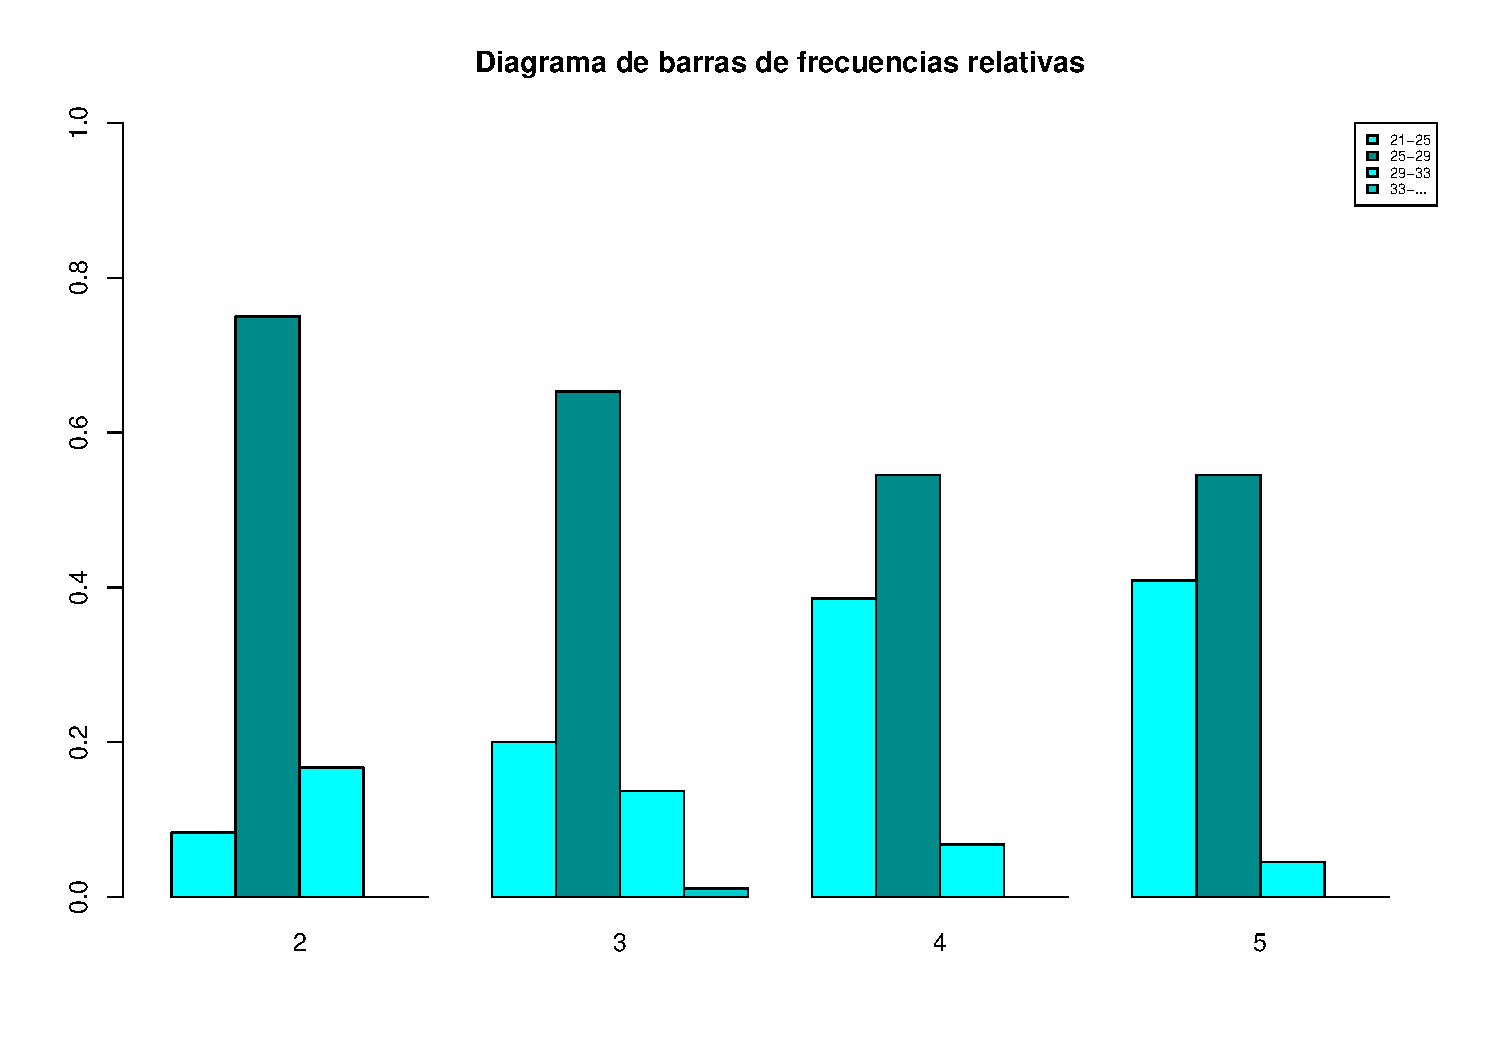
\includegraphics[width=300px]{Hora4_files/figure-beamer/unnamed-chunk-28-1} \end{center}
\end{frame}

\begin{frame}[fragile]{Ejemplo 5}
\protect\hypertarget{ejemplo-5-9}{}
\begin{Shaded}
\begin{Highlighting}[]
\FunctionTok{barplot}\NormalTok{(Fr.rel.acu, }\AttributeTok{beside =} \ConstantTok{TRUE}\NormalTok{, }\AttributeTok{legend =} \ConstantTok{TRUE}\NormalTok{, }\AttributeTok{col =}\NormalTok{ azul, }
        \AttributeTok{main =} \StringTok{"Diagrama de barras de frecuencias relativas acumuladas"}\NormalTok{, }
        \AttributeTok{args.legend=}\FunctionTok{list}\NormalTok{(}\AttributeTok{x =} \StringTok{"topleft"}\NormalTok{, }\AttributeTok{cex=}\FloatTok{0.55}\NormalTok{))}
\end{Highlighting}
\end{Shaded}
\end{frame}

\begin{frame}{Ejemplo 5}
\protect\hypertarget{ejemplo-5-10}{}
\begin{center}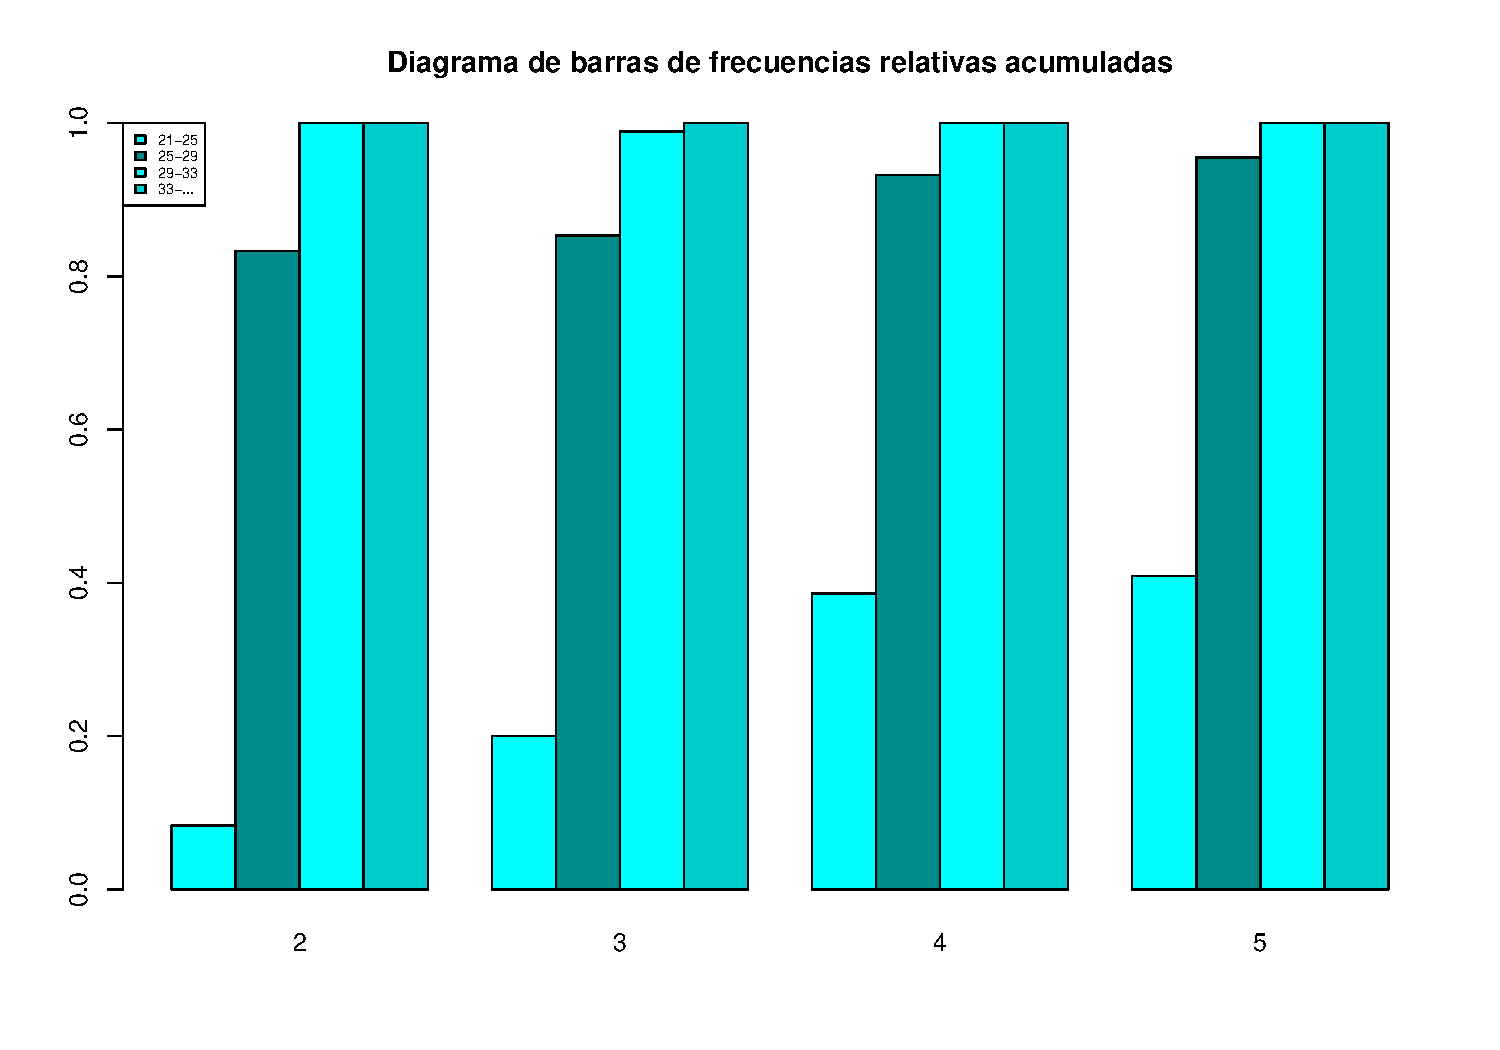
\includegraphics[width=250px]{Hora4_files/figure-beamer/unnamed-chunk-30-1} \end{center}

Los \blue{datos ordinales} son parecidos a los cualitativos, en el
sentido de que son cualidades de los individuos u objetos.

La diferencia existente entre los datos cualitativos y los ordinales
reside en las características que expresan. En el caso de los ordinales,
éstas tienen un orden natural que permite ``acumular'' observaciones.
\end{frame}

\hypertarget{descripciuxf3n-de-datos-cuantitativos}{%
\section{Descripción de datos
cuantitativos}\label{descripciuxf3n-de-datos-cuantitativos}}

\begin{frame}{Datos cuantitativos}
\protect\hypertarget{datos-cuantitativos}{}
Los \blue{datos cuantitativos} son los que expresan cantidades que se
representan mediante números. Éstos se suelen clasificar en continuos y
discretos.

\begin{itemize}
\item
  Los \blue{datos continuos} son los que, si existiese la posibilidad de
  medirlos con precisión infinita, en principio podrían tomar todos los
  valores de un intervalo de la recta real. A modo de ejemplo, el peso,
  la altura, el tiempo\ldots{} son datos de este tipo.
\item
  Por su parte, los \blue{datos discretos} son los que pueden tomar un
  solo conjunto contable de valores. El número de colores de un gato, el
  número de individuos que conforman una población son algunos ejemplos
  de este tipo de datos.
\end{itemize}

Conviene tener en cuenta que esta división es solo teórica. Es decir, en
la práctica, todos estos datos son discretos puesto que la precisión
infinita no existe. Sin embargo, es necesario de vez en cuando suponer
los datos de tipo continuo para así poder utilizar técnicas específicas
en su análisis.
\end{frame}

\begin{frame}{Datos cuantitativos}
\protect\hypertarget{datos-cuantitativos-1}{}
A la hora de estudiar \blue{variables cuantitativas}, podemos utilizar
las frecuencias que hemos visto hasta el momento: absoluta, relativa,
acumulada y relativa acumulada. Esto se debe a que podemos ordenar los
datos cuantitativos en el orden natural de los números reales.

En este caso, disponemos de muchas otras técnicas descriptivas aparte de
las frecuencias, puesto que estamos trabajando con números reales y
podemos operar con ellos.

Los datos cuantitativos admiten dos tipos de tratamiento según
trabajemos con los \blue{raw data} (datos brutos u originales) o bien
los agrupemos en clases o intervalos.

En esta lección trabajaremos sobre la primera situación. En la
siguiente, estudiaremos la descripción de datos cuantitativos agrupados.
\end{frame}

\begin{frame}{Frecuencias de datos cuantitativos}
\protect\hypertarget{frecuencias-de-datos-cuantitativos}{}
El tratamiento de las frecuencias de datos cuantitativos es similar al
de los datos ordinales. La cosa cambia ligeramente debido a que no se
tienen en cuenta todos los niveles posibles, sino únicamente los
observados.
\end{frame}

\begin{frame}[fragile]{Ejemplo 1}
\protect\hypertarget{ejemplo-1-4}{}
\textbf{Ejemplo 1}

Se han pedido las edades a 20 clientes de un museo. Las respuestas
obtenidas han sido las siguientes:

\begin{Shaded}
\begin{Highlighting}[]
\NormalTok{edad }\OtherTok{=} \FunctionTok{c}\NormalTok{(}\DecValTok{15}\NormalTok{,}\DecValTok{18}\NormalTok{,}\DecValTok{25}\NormalTok{,}\DecValTok{40}\NormalTok{,}\DecValTok{30}\NormalTok{,}\DecValTok{29}\NormalTok{,}\DecValTok{56}\NormalTok{,}\DecValTok{40}\NormalTok{,}\DecValTok{13}\NormalTok{,}\DecValTok{27}\NormalTok{,}\DecValTok{42}\NormalTok{,}\DecValTok{23}\NormalTok{,}\DecValTok{11}\NormalTok{,}\DecValTok{26}\NormalTok{,}\DecValTok{25}\NormalTok{,}\DecValTok{32}\NormalTok{,}\DecValTok{30}\NormalTok{,}\DecValTok{40}\NormalTok{,}\DecValTok{33}\NormalTok{,}\DecValTok{29}\NormalTok{)}
\end{Highlighting}
\end{Shaded}

Recordemos que solamente nos interesan las frecuencias de las edades
observadas. Es decir, solamente nos interesan

\begin{Shaded}
\begin{Highlighting}[]
\FunctionTok{table}\NormalTok{(edad)}
\end{Highlighting}
\end{Shaded}

\begin{verbatim}
## edad
## 11 13 15 18 23 25 26 27 29 30 32 33 40 42 56 
##  1  1  1  1  1  2  1  1  2  2  1  1  3  1  1
\end{verbatim}
\end{frame}

\begin{frame}[fragile]{Ejemplo 1}
\protect\hypertarget{ejemplo-1-5}{}
Calculemos el resto de frecuencias como ya sabemos

\begin{Shaded}
\begin{Highlighting}[]
\FunctionTok{round}\NormalTok{(}\FunctionTok{prop.table}\NormalTok{(}\FunctionTok{table}\NormalTok{(edad)),}\DecValTok{3}\NormalTok{)}
\end{Highlighting}
\end{Shaded}

\begin{verbatim}
## edad
##   11   13   15   18   23   25   26   27   29   30   32   33   40   42   56 
## 0.05 0.05 0.05 0.05 0.05 0.10 0.05 0.05 0.10 0.10 0.05 0.05 0.15 0.05 0.05
\end{verbatim}

\begin{Shaded}
\begin{Highlighting}[]
\FunctionTok{cumsum}\NormalTok{(}\FunctionTok{table}\NormalTok{(edad))}
\end{Highlighting}
\end{Shaded}

\begin{verbatim}
## 11 13 15 18 23 25 26 27 29 30 32 33 40 42 56 
##  1  2  3  4  5  7  8  9 11 13 14 15 18 19 20
\end{verbatim}
\end{frame}

\begin{frame}[fragile]{Ejemplo 1}
\protect\hypertarget{ejemplo-1-6}{}
\begin{Shaded}
\begin{Highlighting}[]
\FunctionTok{round}\NormalTok{(}\FunctionTok{cumsum}\NormalTok{(}\FunctionTok{prop.table}\NormalTok{(}\FunctionTok{table}\NormalTok{(edad))),}\DecValTok{3}\NormalTok{)}
\end{Highlighting}
\end{Shaded}

\begin{verbatim}
##   11   13   15   18   23   25   26   27   29   30   32   33   40   42   56 
## 0.05 0.10 0.15 0.20 0.25 0.35 0.40 0.45 0.55 0.65 0.70 0.75 0.90 0.95 1.00
\end{verbatim}
\end{frame}

\begin{frame}{Frecuencias de datos cuantitativos}
\protect\hypertarget{frecuencias-de-datos-cuantitativos-1}{}
En general, supongamos que tenemos \(n\) observaciones de una propiedad
que se mide con un número real y obtenemos la variable cuantitativa
formada por los datos \[x_1,\dots, x_n\]

Sean ahora \(X_1,\dots,X_k\) los valores distintos que aparecen en esta
lista de datos y considerémoslos ordenados \[X_1<X_2<\cdots<X_k\]
\end{frame}

\begin{frame}{Frecuencias de datos cuantitativos}
\protect\hypertarget{frecuencias-de-datos-cuantitativos-2}{}
Entonces, en esta variable cuantitativa

\begin{itemize}
\tightlist
\item
  La frecuencia absoluta de \(X_i\) es el número \(n_i\) de elementos
  que son iguales a \(X_i\)
\item
  La frecuencia relativa de \(X_i\) es \(f_i=\frac{n_i}{n}\)
\item
  La frecuencia absoluta acumulada de \(X_i\) es \(N_i=\sum_{j=1}^in_j\)
\item
  La frecuencia relativa acumulada de \(X_i\) es \(F_i=\frac{N_i}{n}\)
\end{itemize}
\end{frame}

\begin{frame}[fragile]{Ejemplo 2}
\protect\hypertarget{ejemplo-2-2}{}
\textbf{Ejemplo 2}

Lanzamos 25 veces un dado de 6 caras y anotamos las puntuaciones
obtenidas en cada tirada.

En este caso, \(n=25\) y, los distintos valores observados son

\[X_1 = 1,\ X_2 = 2,\ X_3 = 3,\ X_4 = 4,\ X_5 = 5,\ X_6 = 6\]

Nos interesa ahora calcular las frecuencias de este experimento. Además,
las organizaremos en un data frame para observarlas de forma más clara y
sencilla en una tabla.

\begin{Shaded}
\begin{Highlighting}[]
\FunctionTok{set.seed}\NormalTok{(}\DecValTok{162017}\NormalTok{)}
\NormalTok{dados }\OtherTok{=} \FunctionTok{sample}\NormalTok{(}\DecValTok{1}\SpecialCharTok{:}\DecValTok{6}\NormalTok{,}\DecValTok{25}\NormalTok{,}\AttributeTok{replace =} \ConstantTok{TRUE}\NormalTok{)}
\NormalTok{dados}
\end{Highlighting}
\end{Shaded}

\begin{verbatim}
##  [1] 1 1 5 5 5 5 1 6 5 4 1 3 1 3 2 2 1 1 1 4 2 1 6 3 1
\end{verbatim}

\begin{Shaded}
\begin{Highlighting}[]
\FunctionTok{set.seed}\NormalTok{(}\ConstantTok{NULL}\NormalTok{)}
\end{Highlighting}
\end{Shaded}
\end{frame}

\begin{frame}[fragile]{Ejemplo 2}
\protect\hypertarget{ejemplo-2-3}{}
\begin{Shaded}
\begin{Highlighting}[]
\FunctionTok{table}\NormalTok{(dados)}
\end{Highlighting}
\end{Shaded}

\begin{verbatim}
## dados
##  1  2  3  4  5  6 
## 10  3  3  2  5  2
\end{verbatim}

\begin{Shaded}
\begin{Highlighting}[]
\FunctionTok{round}\NormalTok{(}\FunctionTok{prop.table}\NormalTok{(}\FunctionTok{table}\NormalTok{(dados)),}\DecValTok{2}\NormalTok{)}
\end{Highlighting}
\end{Shaded}

\begin{verbatim}
## dados
##    1    2    3    4    5    6 
## 0.40 0.12 0.12 0.08 0.20 0.08
\end{verbatim}

\begin{Shaded}
\begin{Highlighting}[]
\FunctionTok{cumsum}\NormalTok{(}\FunctionTok{table}\NormalTok{(dados))}
\end{Highlighting}
\end{Shaded}

\begin{verbatim}
##  1  2  3  4  5  6 
## 10 13 16 18 23 25
\end{verbatim}
\end{frame}

\begin{frame}[fragile]{Ejemplo 2}
\protect\hypertarget{ejemplo-2-4}{}
\begin{Shaded}
\begin{Highlighting}[]
\FunctionTok{round}\NormalTok{(}\FunctionTok{cumsum}\NormalTok{(}\FunctionTok{prop.table}\NormalTok{(}\FunctionTok{table}\NormalTok{(dados))),}\DecValTok{2}\NormalTok{)}
\end{Highlighting}
\end{Shaded}

\begin{verbatim}
##    1    2    3    4    5    6 
## 0.40 0.52 0.64 0.72 0.92 1.00
\end{verbatim}

\begin{Shaded}
\begin{Highlighting}[]
\NormalTok{dados.df }\OtherTok{=} \FunctionTok{data.frame}\NormalTok{(}
  \AttributeTok{Puntuacion =} \DecValTok{1}\SpecialCharTok{:}\DecValTok{6}\NormalTok{,}
  \AttributeTok{Fr.abs =} \FunctionTok{as.vector}\NormalTok{(}\FunctionTok{table}\NormalTok{(dados)),}
  \AttributeTok{Fr.rel =} \FunctionTok{as.vector}\NormalTok{(}\FunctionTok{round}\NormalTok{(}\FunctionTok{prop.table}\NormalTok{(}\FunctionTok{table}\NormalTok{(dados)),}\DecValTok{2}\NormalTok{)),}
  \AttributeTok{Fr.acu =} \FunctionTok{as.vector}\NormalTok{(}\FunctionTok{cumsum}\NormalTok{(}\FunctionTok{table}\NormalTok{(dados))),}
  \AttributeTok{Fr.racu =} \FunctionTok{as.vector}\NormalTok{(}\FunctionTok{round}\NormalTok{(}\FunctionTok{cumsum}\NormalTok{(}
    \FunctionTok{prop.table}\NormalTok{(}\FunctionTok{table}\NormalTok{(dados))),}\DecValTok{2}\NormalTok{)))}
\end{Highlighting}
\end{Shaded}
\end{frame}

\begin{frame}[fragile]{Ejemplo 2}
\protect\hypertarget{ejemplo-2-5}{}
\begin{Shaded}
\begin{Highlighting}[]
\NormalTok{dados.df}
\end{Highlighting}
\end{Shaded}

\begin{verbatim}
##   Puntuacion Fr.abs Fr.rel Fr.acu Fr.racu
## 1          1     10   0.40     10    0.40
## 2          2      3   0.12     13    0.52
## 3          3      3   0.12     16    0.64
## 4          4      2   0.08     18    0.72
## 5          5      5   0.20     23    0.92
## 6          6      2   0.08     25    1.00
\end{verbatim}

¡OJO! Para entrar una tabla unidimensional como una variable en un data
frame, es conveniente transformarla en vector con \texttt{as.vector}. Si
no, cada \texttt{table} y cada \texttt{prop.table} añadirían una columna
extra con los nombres de los niveles.
\end{frame}

\hypertarget{medidas-de-tendencia-central}{%
\section{Medidas de tendencia
central}\label{medidas-de-tendencia-central}}

\begin{frame}{Medidas de tendencia central}
\protect\hypertarget{medidas-de-tendencia-central-1}{}
Las \textbf{medidas de tendencia central} son las que dan un valor
representativo a todas las observaciones. Algunas de las más importantes
son:

\begin{itemize}
\tightlist
\item
  La \textbf{media aritmética} o \textbf{valor medio}
  \[\bar{x} = \frac{\sum_{i=1}^nx_i}{n}=\frac{\sum_{j=1}^kn_jX_j}{n}=\sum_{j=1}^kf_jX_j\]
\item
  La \textbf{mediana}, que representa el valor central en la lista
  ordenada de observaciones.
\item
  La \textbf{moda} es el valor (o valores) de máxima frecuencia
  (absoluta o relativa, el resultado será el mismo).
\end{itemize}
\end{frame}

\begin{frame}{La mediana}
\protect\hypertarget{la-mediana}{}
La definición formal de la mediana es la siguiente. Denotando por
\[x_{(1)}\le x_{(2)}\le\dots\le x_{(n)}\] los datos de la variable
cuantitativa ordenados de menor a mayor, la mediana es

\begin{itemize}
\tightlist
\item
  Si \(n\) par, la medio de los dos datos centrales
  \[\frac{x_{(\frac{n}{2})}+x_{(\frac{n}{2}+1)}}{2}\]
\item
  Si \(n\) impar, el dato central \(x_{(\frac{n+1}{2})}\)
\end{itemize}
\end{frame}

\begin{frame}[fragile]{Ejemplo 1}
\protect\hypertarget{ejemplo-1-7}{}
Recordemos el ejemplo de las edades.

\begin{Shaded}
\begin{Highlighting}[]
\FunctionTok{sort}\NormalTok{(edad) }\CommentTok{\#Ordenamos los datos por su orden natural}
\end{Highlighting}
\end{Shaded}

\begin{verbatim}
##  [1] 11 13 15 18 23 25 25 26 27 29 29 30 30 32 33 40 40 40 42 56
\end{verbatim}

\begin{Shaded}
\begin{Highlighting}[]
\FunctionTok{table}\NormalTok{(edad)}
\end{Highlighting}
\end{Shaded}

\begin{verbatim}
## edad
## 11 13 15 18 23 25 26 27 29 30 32 33 40 42 56 
##  1  1  1  1  1  2  1  1  2  2  1  1  3  1  1
\end{verbatim}

En este caso, la moda es 40, la mediana es \(\frac{29+29}{2}=29\) y la
media aritmética es

\begin{align*}
& \frac{11+13+15+18+23+25+25+26+27+29+29+30+30+32+33+40+40+40+42+56}{20}  \\  &= 29.2
\end{align*}
\end{frame}

\begin{frame}[fragile]{Ejemplo 2}
\protect\hypertarget{ejemplo-2-6}{}
Recordemos el ejemplo de los dados.

\begin{Shaded}
\begin{Highlighting}[]
\NormalTok{dados.df}
\end{Highlighting}
\end{Shaded}

\begin{verbatim}
##   Puntuacion Fr.abs Fr.rel Fr.acu Fr.racu
## 1          1     10   0.40     10    0.40
## 2          2      3   0.12     13    0.52
## 3          3      3   0.12     16    0.64
## 4          4      2   0.08     18    0.72
## 5          5      5   0.20     23    0.92
## 6          6      2   0.08     25    1.00
\end{verbatim}

En este caso, la moda son dos valores: el 2 y el 3. La mediana es
\(x_{(13)}=\) 3 y la media aritmética es 2.8
\end{frame}

\begin{frame}[fragile]{Medidas de tendencia central en R}
\protect\hypertarget{medidas-de-tendencia-central-en-r}{}
Vamos a calcular la media aritmética, mediana y moda de los dos ejemplos
anteriores con instrucciones de R.

\begin{Shaded}
\begin{Highlighting}[]
\FunctionTok{mean}\NormalTok{(edad) }\CommentTok{\#La media aritmética}
\end{Highlighting}
\end{Shaded}

\begin{verbatim}
## [1] 29.2
\end{verbatim}

\begin{Shaded}
\begin{Highlighting}[]
\FunctionTok{mean}\NormalTok{(dados)}
\end{Highlighting}
\end{Shaded}

\begin{verbatim}
## [1] 2.8
\end{verbatim}

\begin{Shaded}
\begin{Highlighting}[]
\FunctionTok{median}\NormalTok{(edad) }\CommentTok{\#La mediana}
\end{Highlighting}
\end{Shaded}

\begin{verbatim}
## [1] 29
\end{verbatim}
\end{frame}

\begin{frame}[fragile]{Medidas de tendencia central en R}
\protect\hypertarget{medidas-de-tendencia-central-en-r-1}{}
\begin{Shaded}
\begin{Highlighting}[]
\FunctionTok{median}\NormalTok{(dados)}
\end{Highlighting}
\end{Shaded}

\begin{verbatim}
## [1] 2
\end{verbatim}

\begin{Shaded}
\begin{Highlighting}[]
\FunctionTok{as.numeric}\NormalTok{(}\FunctionTok{names}\NormalTok{(}\FunctionTok{which}\NormalTok{(}
  \FunctionTok{table}\NormalTok{(edad)}\SpecialCharTok{==}\FunctionTok{max}\NormalTok{(}\FunctionTok{table}\NormalTok{(edad))))) }\CommentTok{\#La moda}
\end{Highlighting}
\end{Shaded}

\begin{verbatim}
## [1] 40
\end{verbatim}

\begin{Shaded}
\begin{Highlighting}[]
\FunctionTok{as.numeric}\NormalTok{(}\FunctionTok{names}\NormalTok{(}\FunctionTok{which}\NormalTok{(}
  \FunctionTok{table}\NormalTok{(dados)}\SpecialCharTok{==}\FunctionTok{max}\NormalTok{(}\FunctionTok{table}\NormalTok{(dados)))))}
\end{Highlighting}
\end{Shaded}

\begin{verbatim}
## [1] 1
\end{verbatim}

Cuando trabajamos con datos cuantitativos, es conveniente que el
resultado lo demos como un número. De ahí que hayamos aplicado la
función \texttt{as.numeric}.
\end{frame}

\hypertarget{medidas-de-posiciuxf3n}{%
\section{Medidas de posición}\label{medidas-de-posiciuxf3n}}

\begin{frame}{Medidas de posición}
\protect\hypertarget{medidas-de-posiciuxf3n-1}{}
Las \blue{medidas de posición} estiman qué valores dividen las
observaciones en unas determinadas proporciones.

Los valores que determinan estas posiciones son conocidos como los
\blue{cuantiles}.

Pensándolo de este modo, la mediana puede interpretarse como una medida
de posición, debido a que divide la variable cuantitativa en dos
mitades.
\end{frame}

\begin{frame}{Medidas de posición}
\protect\hypertarget{medidas-de-posiciuxf3n-2}{}
Dada una proporción \(p\in(0,1)\), el \blue{cuantil de orden $p$} de una
variable cuantitativa, \(Q_p\), es el valor más pequeño tal que su
frecuencia relativa acumulada es mayor o igual a \(p\).

Dicho de otro modo, si tenemos un conjunto de observaciones
\(x_1,\dots,x_n\) y los ordenamos de menor a mayor, entonces \(Q_p\)
será el número más pequeño que deja a su izquierda (incluyéndose a sí
mismo) como mínimo a la fracción \(p\) de los datos. Es decir,
\(p\cdot n\).

Así, ahora es más claro ver que la mediana vendría a ser \(Q_{0.5}\), el
cuantil de orden 0.5.
\end{frame}

\begin{frame}[fragile]{Ejemplo 3}
\protect\hypertarget{ejemplo-3-5}{}
\textbf{Ejemplo 3}

Consideremos un experimento en el que lanzamos 50 veces un dado de 4
caras y obtenemos los siguientes resultados

\begin{Shaded}
\begin{Highlighting}[]
\FunctionTok{set.seed}\NormalTok{(}\DecValTok{260798}\NormalTok{)}
\NormalTok{dado }\OtherTok{=} \FunctionTok{sample}\NormalTok{(}\DecValTok{1}\SpecialCharTok{:}\DecValTok{4}\NormalTok{, }\DecValTok{50}\NormalTok{, }\AttributeTok{replace =} \ConstantTok{TRUE}\NormalTok{)}
\FunctionTok{set.seed}\NormalTok{(}\ConstantTok{NULL}\NormalTok{)}
\FunctionTok{length}\NormalTok{(dado)}
\end{Highlighting}
\end{Shaded}

\begin{verbatim}
## [1] 50
\end{verbatim}

\begin{Shaded}
\begin{Highlighting}[]
\NormalTok{dado }\OtherTok{=} \FunctionTok{sort}\NormalTok{(dado) }\CommentTok{\#Los ordenamos de menor a mayor}
\NormalTok{dado}
\end{Highlighting}
\end{Shaded}

\begin{verbatim}
##  [1] 1 1 1 1 1 1 1 1 1 1 1 1 1 1 1 1 2 2 2 2 2 2 2 2 2 2 2 2 2 2 2 3 3 3 3 3 4 4
## [39] 4 4 4 4 4 4 4 4 4 4 4 4
\end{verbatim}
\end{frame}

\begin{frame}[fragile]{Ejemplo 3}
\protect\hypertarget{ejemplo-3-6}{}
\begin{Shaded}
\begin{Highlighting}[]
\NormalTok{df.dado }\OtherTok{=} \FunctionTok{data.frame}\NormalTok{(}
  \AttributeTok{Puntuacion =} \DecValTok{1}\SpecialCharTok{:}\DecValTok{4}\NormalTok{,}
  \AttributeTok{Fr.abs =} \FunctionTok{as.vector}\NormalTok{(}\FunctionTok{table}\NormalTok{(dado)),}
  \AttributeTok{Fr.rel =} \FunctionTok{as.vector}\NormalTok{(}\FunctionTok{round}\NormalTok{(}\FunctionTok{prop.table}\NormalTok{(}\FunctionTok{table}\NormalTok{(dado)),}\DecValTok{2}\NormalTok{)),}
  \AttributeTok{Fr.acu =} \FunctionTok{as.vector}\NormalTok{(}\FunctionTok{cumsum}\NormalTok{(}\FunctionTok{table}\NormalTok{(dado))),}
  \AttributeTok{Fr.racu =} \FunctionTok{as.vector}\NormalTok{(}\FunctionTok{round}\NormalTok{(}\FunctionTok{cumsum}\NormalTok{(}
    \FunctionTok{prop.table}\NormalTok{(}\FunctionTok{table}\NormalTok{(dado))),}\DecValTok{2}\NormalTok{))}
\NormalTok{  )}
\NormalTok{df.dado}
\end{Highlighting}
\end{Shaded}

\begin{verbatim}
##   Puntuacion Fr.abs Fr.rel Fr.acu Fr.racu
## 1          1     16   0.32     16    0.32
## 2          2     15   0.30     31    0.62
## 3          3      5   0.10     36    0.72
## 4          4     14   0.28     50    1.00
\end{verbatim}
\end{frame}

\begin{frame}{Ejemplo 3}
\protect\hypertarget{ejemplo-3-7}{}
Si nos piden el cuantil \(Q_{0.3}\), sabemos que este es el primer
elemento de la lista cuya frecuencia relativa acumulada es mayor o igual
a 0.3. Este se corresponde con la puntuación 1.
\end{frame}

\begin{frame}[fragile]{Ejemplo 3}
\protect\hypertarget{ejemplo-3-8}{}
También podríamos hallarlo de otro modo: fijándonos en la lista ordenada
de puntuaciones, el cuantil \(Q_{0.3}\) sería el primer elemento de
dicha lista tal que fuera mayor o igual que, como mínimo, el 30\% de los
datos. Si calculamos el 30\% de 50, obtenemos que es 15. Esto lo que nos
dice es que el cuantil que buscamos es el número que se encuentra en la
quinceava posición de la lista ordenada.

\begin{Shaded}
\begin{Highlighting}[]
\NormalTok{dado[}\DecValTok{15}\NormalTok{]}
\end{Highlighting}
\end{Shaded}

\begin{verbatim}
## [1] 1
\end{verbatim}
\end{frame}

\begin{frame}{Cuantiles}
\protect\hypertarget{cuantiles}{}
Algunos cuantiles tienen nombre propio:

\begin{itemize}
\tightlist
\item
  Los \textbf{cuartiles} son los cuantiles \(Q_{0.25},Q_{0.5}\) y
  \(Q_{0.75}\). Respectivamente, son llamados primer, segundo y tercer
  cuartil. El primer cuartil, \(Q_{0.25}\), será el menor valor que es
  mayor o igual a una cuarta parte de las observaciones y \(Q_{0.75}\),
  el menor valor que es mayor o igual a tres cuartas partes de los datos
  observados.
\item
  El cuantil \(Q_{0.5}\) es la mediana
\item
  Los \textbf{deciles} son los cuantiles \(Q_p\) con \(p\) un múltiplo
  de 0.1.
\item
  Los \textbf{percentiles} son son los cuantiles \(Q_p\) con \(p\) un
  múltiplo de 0.01.
\end{itemize}
\end{frame}

\begin{frame}[fragile]{Cuantiles}
\protect\hypertarget{cuantiles-1}{}
La definición de cuantil anteriormente dada es orientativa. La realidad
es que, exceptuando el caso de la mediana, no hay consenso sobre cómo
deben calcularse los cuantiles. En verdad, existen diferentes métodos
que pueden dar lugar a soluciones distintas.

Al fin y al cabo, nuestro objetivo no es el de encontrar el primer valor
de una muestra cuya frecuencia relativa acumulada en la variable sea
mayor o igual a \(p\), sino estimar el valor de esta cantidad para el
total de la población.

Para calcular los cuantiles de orden \(p\) de una variable cualitativa
\(x\) con R, se utiliza la instrucción \texttt{quantile(x,p)}, la cual
dispone de 9 métodos diferentes que se especifican con el parámetro
\texttt{type}. El valor por defecto es \texttt{type\ =\ 7} y no hace
falta especificarlo, como veremos en el siguiente ejemplo. Para más
información sobre todos los valores posibles de este parámetro, haced
click en el enlace a
\href{https://es.wikipedia.org/wiki/Cuantil}{Wikipedia}
\end{frame}

\begin{frame}[fragile]{Ejemplo 4}
\protect\hypertarget{ejemplo-4-8}{}
\begin{Shaded}
\begin{Highlighting}[]
\FunctionTok{set.seed}\NormalTok{(}\DecValTok{0}\NormalTok{)}
\NormalTok{dados2 }\OtherTok{=} \FunctionTok{sample}\NormalTok{(}\DecValTok{1}\SpecialCharTok{:}\DecValTok{6}\NormalTok{,}\DecValTok{15}\NormalTok{, }\AttributeTok{replace =} \ConstantTok{TRUE}\NormalTok{)}
\NormalTok{dados2}
\end{Highlighting}
\end{Shaded}

\begin{verbatim}
##  [1] 6 1 4 1 2 5 3 6 2 3 3 1 5 5 2
\end{verbatim}

\begin{Shaded}
\begin{Highlighting}[]
\FunctionTok{set.seed}\NormalTok{(}\ConstantTok{NULL}\NormalTok{)}
\FunctionTok{quantile}\NormalTok{(dados2,}\FloatTok{0.25}\NormalTok{) }\CommentTok{\#Primer cuartil}
\end{Highlighting}
\end{Shaded}

\begin{verbatim}
## 25% 
##   2
\end{verbatim}

\begin{Shaded}
\begin{Highlighting}[]
\FunctionTok{quantile}\NormalTok{(dados2,}\FloatTok{0.8}\NormalTok{)}
\end{Highlighting}
\end{Shaded}

\begin{verbatim}
## 80% 
##   5
\end{verbatim}
\end{frame}

\end{document}
